\documentclass[12pt,a4paper,spanish]{article}
\usepackage[margin=2.54cm,]{geometry}
\usepackage[pdftex]{graphicx}
\usepackage{pdfpages}
\usepackage{color}
\usepackage{listing}
\usepackage{listings}
\usepackage{dirtree}
\usepackage{float}
\usepackage{hyperref}
\usepackage{ulem}
\usepackage{xcolor}
\usepackage{listingsutf8}
\usepackage{titlesec}
\usepackage{etoolbox}
\usepackage{afterpage}
\usepackage[utf8]{inputenc}
\usepackage[toc,acronym]{glossaries}
\usepackage[noabbrev,capitalise,nameinlink]{cleveref}
\hypersetup{colorlinks={true},linkcolor={blue},citecolor=green}
\usepackage{caption}

\makenoidxglossaries
\newglossaryentry{API}{name={API},description={(Application Programming Interface) Conjunto de reglas y protocolos de programación que especifican cómo los componentes de software deben interactuar entre sí sin tener que conocer los detalles subyacentes de implementación}}
\newglossaryentry{REST}{name={REST},description={(Representational State Transfer) es un estilo de arquitectura de software para sistemas distribuidos que se utiliza para diseñar servicios web que son fáciles de escalar, mantener y extender}}
\newglossaryentry{RPC}{name={RPC},description={(Remote Procedure Call) Protocolo de comunicación utilizado en sistemas distribuidos que permite que un programa solicite servicios o funciones a través de la red a otro programa en una máquina remota.}}
\newglossaryentry{CRUD}{name={CRUD},description={Acrónimo de las cuatro operaciones básicas en la gestión de datos: Crear (Create), Leer (Read), Actualizar (Update) y Eliminar (Delete)}}
\newglossaryentry{Backend}{name={Backend},description={Conjunto de servidores, aplicaciones y servicios que se ejecutan en segundo plano y proporcionan una interfaz de programación de aplicaciones (API) para que los clientes (front-end) puedan interactuar con ellos}}
\newglossaryentry{Manager} {name={Manager},description={Servicio web o Backend diseñado en este TFM para la gestión de tareas}}
\newglossaryentry{Client} {name={Client},description={Servicio web o Backend diseñado en este TFM para la ejecucion de tareas albergados en sistemas remotos}}
\newglossaryentry{LayerArchitecture} {name={Layered Architecture},description={(Arquitectura de capas) es un enfoque de diseño de software en el que los componentes del sistema se dividen en capas lógicas y se comunican entre sí a través de interfaces definidas}}
\newglossaryentry{HexagonalArchitecture} {name={Hexagonal Architecture},description={(Arquitectura hexagonal o arquitectura de puertos y adaptadores) Implementación concreta de la arquitectura de capas.
Basada en el diseño de un núcleo del sistema (Dominio) independiente de su entorno con el que se comunican los agentes externos a través de puertos y adaptadores}}
\newglossaryentry{DDD} {name={DDD},description={(Domain-Driven Design o Diseño Dirigido por el Dominio) capa central en arquitectura de capas o hexagonal.
Entidades, objetos, conceptos y relaciones que conforman el núcleo del negocio.
Refleja y dar soporte al negocio que se está modelando.
Define un lenguaje común (ubiquitous language) que se comparte entre los expertos del dominio de la aplicación y los desarrolladores de software}}
\newglossaryentry{CQRS} {name={CQRS},description={(Command Query Responsibility Segregation) Segregación de responsabilidades de comandos y consultas.
Es una técnica de diseño de arquitectura de software que separa la lógica de escritura (comandos) de la lógica de lectura (consultas) en sistemas de información}}
\newglossaryentry{Entity} {name={Entity},description={(Entidad) Es un objeto de Dominio que tiene identidad única y representa un concepto del mundo real, del negocio.
Pueden ser almacenados, recuperados y modificados en la base de datos}}
\newglossaryentry{Value Object} {name={ValueObject},description={(Objeto de valor) Representa la descripción de un objeto, pero no tiene identidad propia.
Son inmutables.
Se utilizan para representar datos que no necesitan ser almacenados individualmente en base de datos}}
\newglossaryentry{Service} {name={Service},description={(Servicio) Componente software que proporciona funcionalidades y operaciones que no están directamente relacionadas con ninguna entidad o valor específico.
Los servicios encapsulan la lógica de negocio compleja y se utilizan para ejecutar operaciones que involucran múltiples entidades o valores}}
\newglossaryentry{Repository} {name={Repository},description={(Repositorio) Es un objeto que proporciona una interfaz para interactuar con la base de datos y abstrae la lógica de almacenamiento de datos del resto de la aplicación.
Los repositorios se utilizan para realizar operaciones de almacenamiento, recuperación, actualización y eliminación de entidades}}
\newglossaryentry{InfrastructureLayer} {name={Infrastructure Layer},description={(Capa de infraestructura) Proporciona una interfaz para interactuar con componentes como bases de datos, sistemas de archivos o servicios web.
Implementa detalles técnicos que dependen de una tecnología concreta y no deben afectar al modelado del negocio}}
\newglossaryentry{Adapter} {name={Adapter},description={(Adaptador) Elemento de software que implementa una interfaz para conectar la capa de aplicación o dominio con los componentes de infraestructura}}
\newglossaryentry{ApplicationLayer}{ name={Application layer},description={(Capa de aplicación) Capa que contiene los casos de uso específicos del negocio.
Proporciona una interfaz para interactuar con el dominio}}
\newglossaryentry{UseCase} {name={Use Case},description={(Caso de uso) Escenario específico de uso de la aplicación que involucra múltiples operaciones y procesos.
Los casos de uso se utilizan para representar la funcionalidad de la aplicación desde la perspectiva del usuario}}
\newglossaryentry{Command}{name={Comando},description={(Comando) Operación que realiza un cambio en el estado del sistema}}
\newglossaryentry{SUT}{name={SUT},description={System Under Test (Sistema bajo testeo)}}
\newglossaryentry{DOC}{name={DOC},description={Depended On Component (Dependiente del componente)}}
\newglossaryentry{DTO}{name={DTO},description={Data Transfer Object (Objeto de transferencia de datos) Objeto inmutable que sólo sirve para transportar información de una capa a otra}}
\newglossaryentry{UL}{name={UL},description={(Ubiquitous Language) Lenguaje común en un diseño guiado por DDD para describir los componentes del problema}}
\newglossaryentry{IDL}{name={IDL},description={(interface definition language)}}
\newglossaryentry{Query} {name={Command},description={(Consulta) Operación que recupera información del sistema sin modificar su estado}}
\newglossaryentry{E2E} {name={E2E},description={(End to End o extremo a extremo) Tipología de test que prueba todo el sistema}}
\newglossaryentry{CI/CD} {name={CI/CD},description={(Continuous delivery/Continuous integration) Entrega Continua/Integración Continua.
Prácticas y herramientas para automatizar el proceso de garantizar el correcto desarrollo de software desde la creación del código hasta su despliegue en producción}}

\begin{document}
    \titleformat{\paragraph}
{\normalfont\normalsize\bfseries}{\theparagraph}{1em}{}
\titlespacing*{\paragraph}
{0pt}{3.25ex plus 1ex minus .2ex}{1.5ex plus .2ex}
\setlength{\parskip}{\baselineskip}%
\setlength{\parindent}{0pt}%

\newcommand\blankpage{%
    \null
    \thispagestyle{empty}%
    \addtocounter{page}{-1}%
    \newpage}
\patchcmd{\thebibliography}{\section*{\refname}}{}{}{}
\titleformat{\subparagraph}
{\normalfont\normalsize\bfseries}{\thesubparagraph}{1em}{}
\titlespacing*{\subparagraph}
{0pt}{3.25ex plus 1ex minus .2ex}{1.5ex plus .2ex}
\setcounter{tocdepth}{4}
\setcounter{secnumdepth}{4}
\lstset{language=Go,
    basicstyle=\ttfamily\scriptsize,
    keywordstyle=\color{blue}\ttfamily,
    stringstyle=\color{red}\ttfamily,
    commentstyle=\color{green}\ttfamily}

\lstdefinelanguage{docker}{
    keywords={FROM, RUN, COPY, ADD, ENTRYPOINT, CMD,  ENV, ARG, WORKDIR, EXPOSE, LABEL, USER, VOLUME, STOPSIGNAL, ONBUILD, MAINTAINER},
    keywordstyle=\color{blue}\bfseries,
    identifierstyle=\color{black},
    sensitive=false,
    comment=[l]{\#},
    commentstyle=\color{purple}\ttfamily,
    stringstyle=\color{red}\ttfamily,
    morestring=[b]',
    morestring=[b]"
}

\lstdefinelanguage{docker-compose}{
    keywords={image, environment, ports, container_name, ports, volumes, links},
    keywordstyle=\color{blue}\bfseries,
    identifierstyle=\color{black},
    sensitive=false,
    comment=[l]{\#},
    commentstyle=\color{purple}\ttfamily,
    stringstyle=\color{red}\ttfamily,
    morestring=[b]',
    morestring=[b]"
}
\lstdefinelanguage{docker-compose-2}{
    keywords={version, volumes, services},
    keywordstyle=\color{blue}\bfseries,
    keywords=[2]{image, environment, ports, container_name, ports, links, build},
    keywordstyle=[2]\color{olive}\bfseries,
    identifierstyle=\color{black},
    sensitive=false,
    comment=[l]{\#},
    commentstyle=\color{purple}\ttfamily,
    stringstyle=\color{red}\ttfamily,
    morestring=[b]',
    morestring=[b]"
}

\lstset{basicstyle=\ttfamily,
    showstringspaces=false,
    commentstyle=\color{red},
    keywordstyle=\color{blue},
    inputencoding=utf8,
    extendedchars=true
}

\crefname{paragraph}{paragraph}{paragraphs}
    

\renewcommand{\contentsname}{Índice General}
\renewcommand{\listtablename}{Lista de Tablas}
\renewcommand{\tablename}{Tabla}

\begin{figure}[H]
        \hspace{-0.5cm}	
		
\includegraphics[scale=0.25]{./1-Portada/img/logoUma}
		\hspace{6cm}
		
\includegraphics[scale= 0.25]{./1-Portada/img/logoEscuela}\label{fig:figure3}
\end{figure}
\vspace*{0.2in}
\begin{center}
	\begin{large}
		\textbf {Escuela de Ingenierías Industriales\\}
	\end{large}	
	\vspace*{0.5cm}
	\begin{large}
		\textbf {Departamento\\ de Ingeniería de Sistemas y Automática\\}
	\end{large}	
	\vspace*{1cm}
	\begin{large}
		\textbf {Área de conocimiento\\Ingeniería de Sistemas y Automática\\}
	\end{large}	
	\vspace*{1cm}	
	\begin{Huge}
		\textbf {Trabajo de Fin de Máster\\}
	\end{Huge}
	\vspace*{0.3cm}
	\begin{LARGE}
		\textbf {Desarrollo de plataforma de control remoto en Golang Go\\}
	\end{LARGE}
	\vspace*{0.3cm}
	\rule{5cm}{0.01cm}\\
	\vspace*{1cm}
	\begin{large}
		\textbf {Autor: Enrique Arrabal Almagro\\}
		\vspace*{0.5cm}
		\textbf {Tutor: Antonio Mandow Andaluz\\}
		\vspace*{1cm}
		\textbf{Titulación: Master en Ingeniería Industrial}
	\end{large}	
	\vspace*{3cm}
\begin{center}
\textbf{}{Málaga, Junio de 2023}
\end{center}					
\end{center}
\thispagestyle{empty}



\newpage
\thispagestyle{empty}
\begin{flushright}
	\phantom{blank}
	\vspace{25mm}

	A mi madre, que me enseñó a soñar \\
	A mi padre, que me enseñó a pensar  \\
	A los que hice daño, por si sirve de algo  \\
	A los que me lo hicieron a mi, porque me enseñó a seguir  \\
	A mi hermanos, en especial a Cris  \\
	Pero sobre todo, Carmina, a tí que me faltas tanto...  \\
\end{flushright}

\includepdf[pages=-]{./part/DeclaracionOriginalidad.pdf}
\tableofcontents
\newpage
\cleardoublepage
	\addcontentsline{lof}{chapter}{Lista de figuras} % para que aparezca en el indice de contenidos
\listoffigures % indice de figuras
\cleardoublepage
	\addcontentsline{lot}{chapter}{Lista de tablas} % para que aparezca en el indice de contenidos
\listoftables % indice de tablas

\newpage	
    \glsaddall
    \printnoidxglossary[style=tree,title=Glosario,nonumberlist]\label{sec:glossary}

    \newpage
    \section{Objetivos}\label{sec:objetivos}
    Desde el punto de vista técnico se va a crear un sistema capaz de albergar y gestionar tareas para su ejecución en remoto.

Para ellos se requerirá un servicio web API (application programming interface) y dos servicios clientes uno para manejarlo el frontend y otro para ejecutar las tareas

Para hacer uso en mayor medidas de la herramienta escogida y para explorar su uso en nuestro campo la tarea a ejecutar en remoto sera un control PID en velocidad y posición de un motor de corriente continua.

Tendremos la capacidad de:

\begin{itemize}
	\item Añadir editar, eliminar y obtener las tareas contenidas en el sistema
	\item Añadir editar, eliminar y obtener los resultados de la ejecución de dichas tareas
	\item Añadir editar, eliminar y obtener las direcciones de los equipos remotos donde se ejecutarán las tareas
\end{itemize} 

El servicio cliente remoto tendrá la capacidad de recibir un comando, ejecutarlo y devolver el resultado.

Desde un punto de vista de gestión del proyecto: se va a hacer uso de las herramientas que se usan en un ámbito profesional para la gestión del mismo dar garantía de calidad, estabilidad, iteración de la solución aportando valor progresivamente evitando desconexión entre el objetivo por parte del cliente y el que ejecuta.

    \newpage
    \section{Resumen}\label{sec:resumen}
    
Se ha diseñado y desarrollado un sistema capaz de gestionar y ejecutar tareas en sistemas remotos.
Como ejemplo de aplicación remota, el sistema consta también de un programa de control PID para un motor de corriente continua.
Respondiendo al objetivo principal se ha obtenido un ejemplo práctico de aplicación de una metodología que abarca el proceso de desarrollo de software, desde su diseño hasta su entrega.
La metodología se basa en un diseño estructurado en capas, separando la solución tecnológica concreta de la lógica que resuelve el problema, facilitando la evolución iterativa del software.
Se ha realizado un esfuerzo de diseño para utilizar un lenguaje expresivo que transmite el problema resuelto.
Dicho lenguaje facilita la comunicación efectiva en todos los participantes del proyecto.
El sistema resultante consta de tres programas independientes:

\begin{itemize}
    \item Un programa que gestiona la interacción entre los distintos sistemas y los usuarios.
    \item Un programa cliente que responde a las ordenes de ejecución de las tareas definidas en el gestor.
    Ejecutable en paralelo en tantas máquinas como se requiera.
    \item Un programa de control PID para ser ejecutado por el cliente.
\end{itemize}

El diseño está enfocado en manejar de forma efectiva el principal problema de desarrollo del software: la evolución.
La evolución y el cambio del software requiere de la interacción entre personas con diferentes conocimientos: técnicos, gente de negocio, clientes y todo aquel afectado.
Personas que comienzan a interactuar con el sistema sin conocimientos previos o gente que deja de interactuar con el mismo eliminando conocimiento del mismo.
También intervienen cambios tecnológicos que no deberían afectar al problema que resuelve.
Por ejemplo, un cambio en el sistema de comunicación, cambiar el uso del correo electrónico a mensajería instantanea no debe suponer un peligro o incertidumbre a la estabilidad de ejecución del sistema.

El presente trabajo evalua cómo responde Golang ante este tipo de proyectos y metodologías.
En particular enfocado a soluciones que requieren de la interacción con actuadores o hardware para el control automático.
Se han puesto a prueba los conceptos clave que el lenguaje promueve: asincronía y gestión de concurrencia y simplicidad.

Se ha realizado el ejercicio de adaptación de los documentos utilizados en un proyecto de ejecución de tipo industrial a un proyecto de software para evaluar su encaje.
Se ha documentado el primer paso del proceso, el diseño, en un documento de proyecto ejecutivo.
Para el segundo paso, el desarrollo, se adapta un documento de ejecución de obra.




    \newpage
    \section{Proyecto Ejecutivo}\label{sec:proyecto_ejecutivo}
    \subsection{Memoria descriptiva}\label{subsec:memoria-descriptiva}
	En el desarrollo de software, el diseño es un proceso iterativo, a diferencia de la construcción de bienes inmuebles. Por lo tanto, la arquitectura del software debe ser flexible para soportar cambios y garantizar que el diseño no obstaculice el proceso iterativo.

Al presentar el diseño inicial, de manera útil para la toma de decisiones a la hora de invertir recursos, es importante explicar su valor y usar una metodología ágil para evitar la parálisis por análisis y no centrarse en detalles técnicos que deben investigarse, analizarse o ponerse a prueba con su propia implementación. El proyecto ejecutivo se entregará como un documento explicativo del diseño, con un equilibrio entre el detalle explicativo para eliminar incertidumbre y la pragmatismo.

En comparación con proyectos industriales, el proyecto de software debe cerrar los aspectos que se puedan cerrar y señalar claramente los puntos de incertidumbre, estimando su costo. El presupuesto indica hasta dónde se puede resolver la incertidumbre. El programa debe entregarse y ser válido únicamente pendiente de resolver la parte afectada para no malgastar recursos. En el lenguaje que vamos a desarrollar se definiría como: dejar el caso de uso desarrollado únicamente pendiente de resolver los adaptadores que cumplan la funcionalidad afectada, pero las reglas del negocio que utilice dicha funcionalidad debe quedar despejada

\subsubsection{Información previa: antecedentes y condiciones}
    
\paragraph{Domain Driven Design}
Se va a proceder a una exposición del vocabulario utilizado en el diseño del software propio de este marco teórico. Las referencias básicas utilizadas para esta exposición de \gls{DDD} son:

\begin{itemize}
    \item Domain-Driven Design: Tackling Complexity in the Heart of Software.\cite{EricEvans2003DDTC}
    \item Implementing Domain-Driven Design.\cite{VaughnVernon2013IDD}
    \item Get Your Hands Dirty on Clean Architecture\cite{TomHombergs2019GYHD}
\end{itemize}

\textit{DDD} es una metodología de diseño enfocada a desarrollar un lenguaje común para todos los partícipes en un problema y su solución por ejemplo: clientes, vendedores, técnicos y financieros en un programa de gestión de venta de productos. Para desarrollar ese lenguaje se divide el problema en contextos delimitados. En un ejemplo rápido: afiliado en un club deportivo significa facturas, números de identificación fiscal para los financieros y para la gente de operaciones significa reserva de pistas y cancelaciones. Para los de ventas significan descuentos, promociones, los demás actores tendrán otro significado para el mismo concepto. pero cuando hablan de afiliados deben entenderse. Si en un departamento lo llaman clientes y en otro afiliados surgen problemas de comunicación. Tener un lenguaje común donde todos puedan expresarse y hablar de la misma solución es el reto de este proceso. Es lo que se define como \gls{UL} Intentar expresar en un mismo contexto todos esos significados termina en lo que se conoce como "Big Ball of Mud" o Gran bola de barro.


Los componentes y las relaciones de este UL se pueden apreciar en la figura~\cref{fig:DomainDrivenDesignReference}.

\begin{figure}[H]
    \centering
    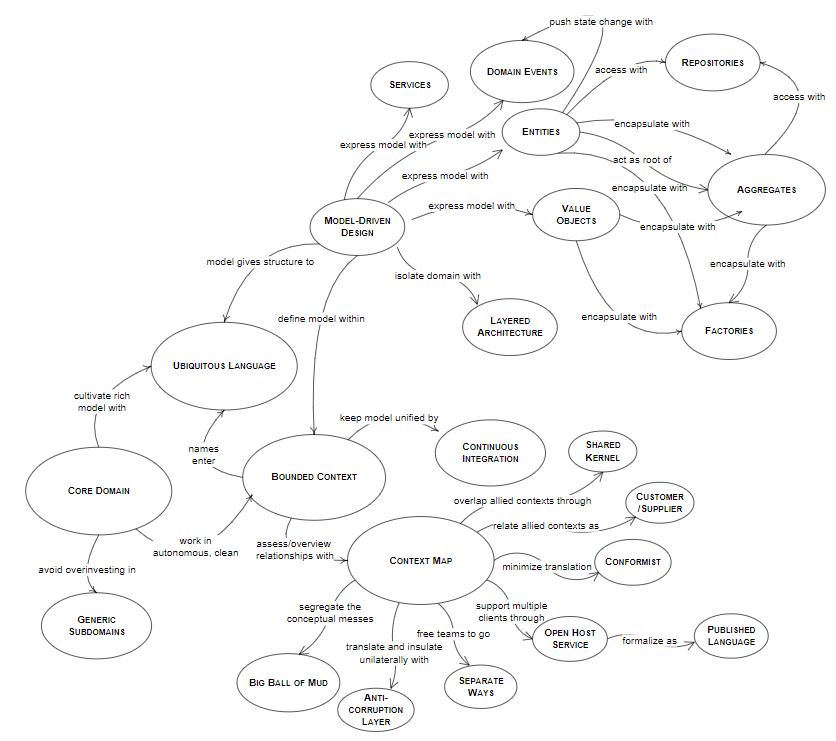
\includegraphics[height=0.5\textheight]{./part/Proyecto_ejecutivo/memoria_descriptiva/infoPreviaAntecedentes/img/DomainDrivenDesignReference}
    \caption{DomainDrivenDesignReference\cite{EricEvans2003DDTC}}\label{fig:DomainDrivenDesignReference}
\end{figure}

De todo este diagrama los conceptos en los que nos vamos a centrar son en los que surgen del componente "Model Driven Design" que son los elementos dentro de ese lenguaje que afectan al diseño del software a su nivel más elemental.

\begin{itemize}
    \item Entity: Elemento que contiene atributos definido por un identificador
    \item \textit{Value Object}: Elemento que tiene atributos pero no identificador
    \item Domain Event: Elemento que define una suceso inducido por la interacción entre los componentes del dominio.
    \item Aggregate: Cluster de elementos tratado como una unidad. Las referencias o acciones externas sobre sus elementos siempre se hacen a través de un único elemento de este cluster conocido como \textit{Agreggate Root}. Tiene reglas definidas de consistencia dentro de su delimitación.
    \item Repository: Es un mecanismo de interaccion para encapsular el acceso a tecnologías, como el almacenamiento en base de datos, para interactuar con ellas. La implementación no concierne al dominio.
    \item Service: Es una funcionalidad de interacción entre elementos de dominio. Encapsula lógica compleja que garantiza un comportamiento consistente.
\end{itemize}

Esta paradigma de diseño compone el elemento central en el paradigma de la arquitectura de capas o \gls{LayerArchitecture}. Se aisla esos contextos que definen nuestro dominio de implementaciones concretas ya sea para acceder al mismo o a las que accede el dominio. Por ejemplo, aislarlo de que se ejecute un servicio mediante una consola de comandos o desde una llamada http y que se guarde en una base de datos la información o se guarde en un archivo.

\paragraph{Hexagonal Architecture}

Dentro de las arquitecturas de capas vamos a utilizar un diseño de puerto y adaptadores o más conocido como \gls{HexagonalArchitecture}. El diagrama básico más utilizado en la teoría para representarlo se muestra en la figura~\cref{fig:hexagonalDiagram}. Como apreciación personal no le encuentro una utilidad real a este tipo de diagramas. El pretendido enfoque didáctico se pierde ya que el hexágono es una simple licencia estética. En el caso de existir más puertos de salida y entrada que los representados, el hexágono pierde todo el sentido. Cuando se enfrenta por primera vez este diagrama se tiende a intentar descifrar el sentído oculto detrás de la elección de la forma poligonal, no existe.

\begin{figure}[H]
    \centering
    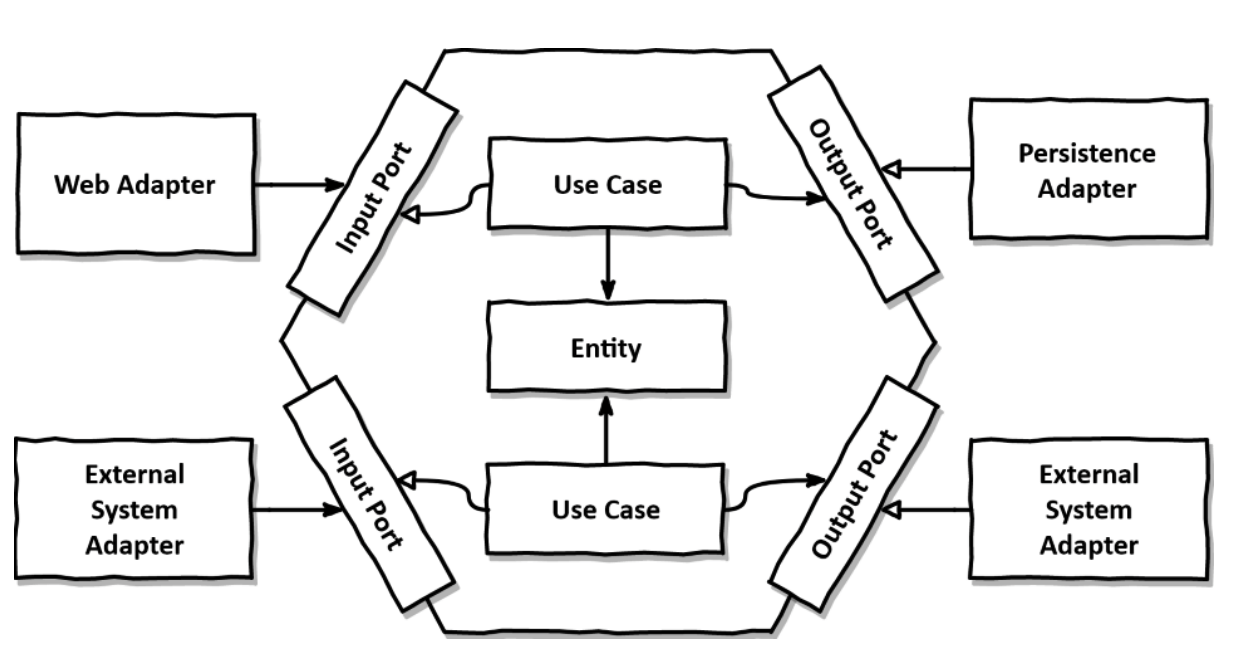
\includegraphics[height=0.3\textheight]{./part/Ejecucion/Seguimiento/CreateTaskUseCase/img/HexagonalDiagram}
    \caption{Hexagonal architecture diagram\cite{TomHombergs2019GYHD}}\label{fig:hexagonalDiagram}
\end{figure}

En este diagrama, el dominio está representado por una única entidad, o Entity, que se encuentra aislada de todo y no depende de ningún elemento. La aplicación está respresentada por los casos de uso, o UseCase, y utiliza el dominio dependiendo de él. La aplicación se aisla del exterior, la infraestructura, obligando a utilizar sus interfaces a los elementos que acceden, esto está representado por la flecha con cabeza hueca o de color blanco. y utilizando interfaces que será responsabilidad de la infraestructura implementar, desconociendo la aplicación su implementación particular.

En el diagrama~\cref{fig:layers} podemos ver este concepto más simplificado. El objetivo es expresar que la dependencia de las capas, expresada por las flechas, sea siempre de fuera hacia adentro. Queremos preservar del cambio el interior y exponer al cambio el exterior. Separar lo propenso al cambio de lo que no. Separar el UL de los detalles de implementación, que tienen su propio lenguaje.

\begin{figure}[H]
    \centering
    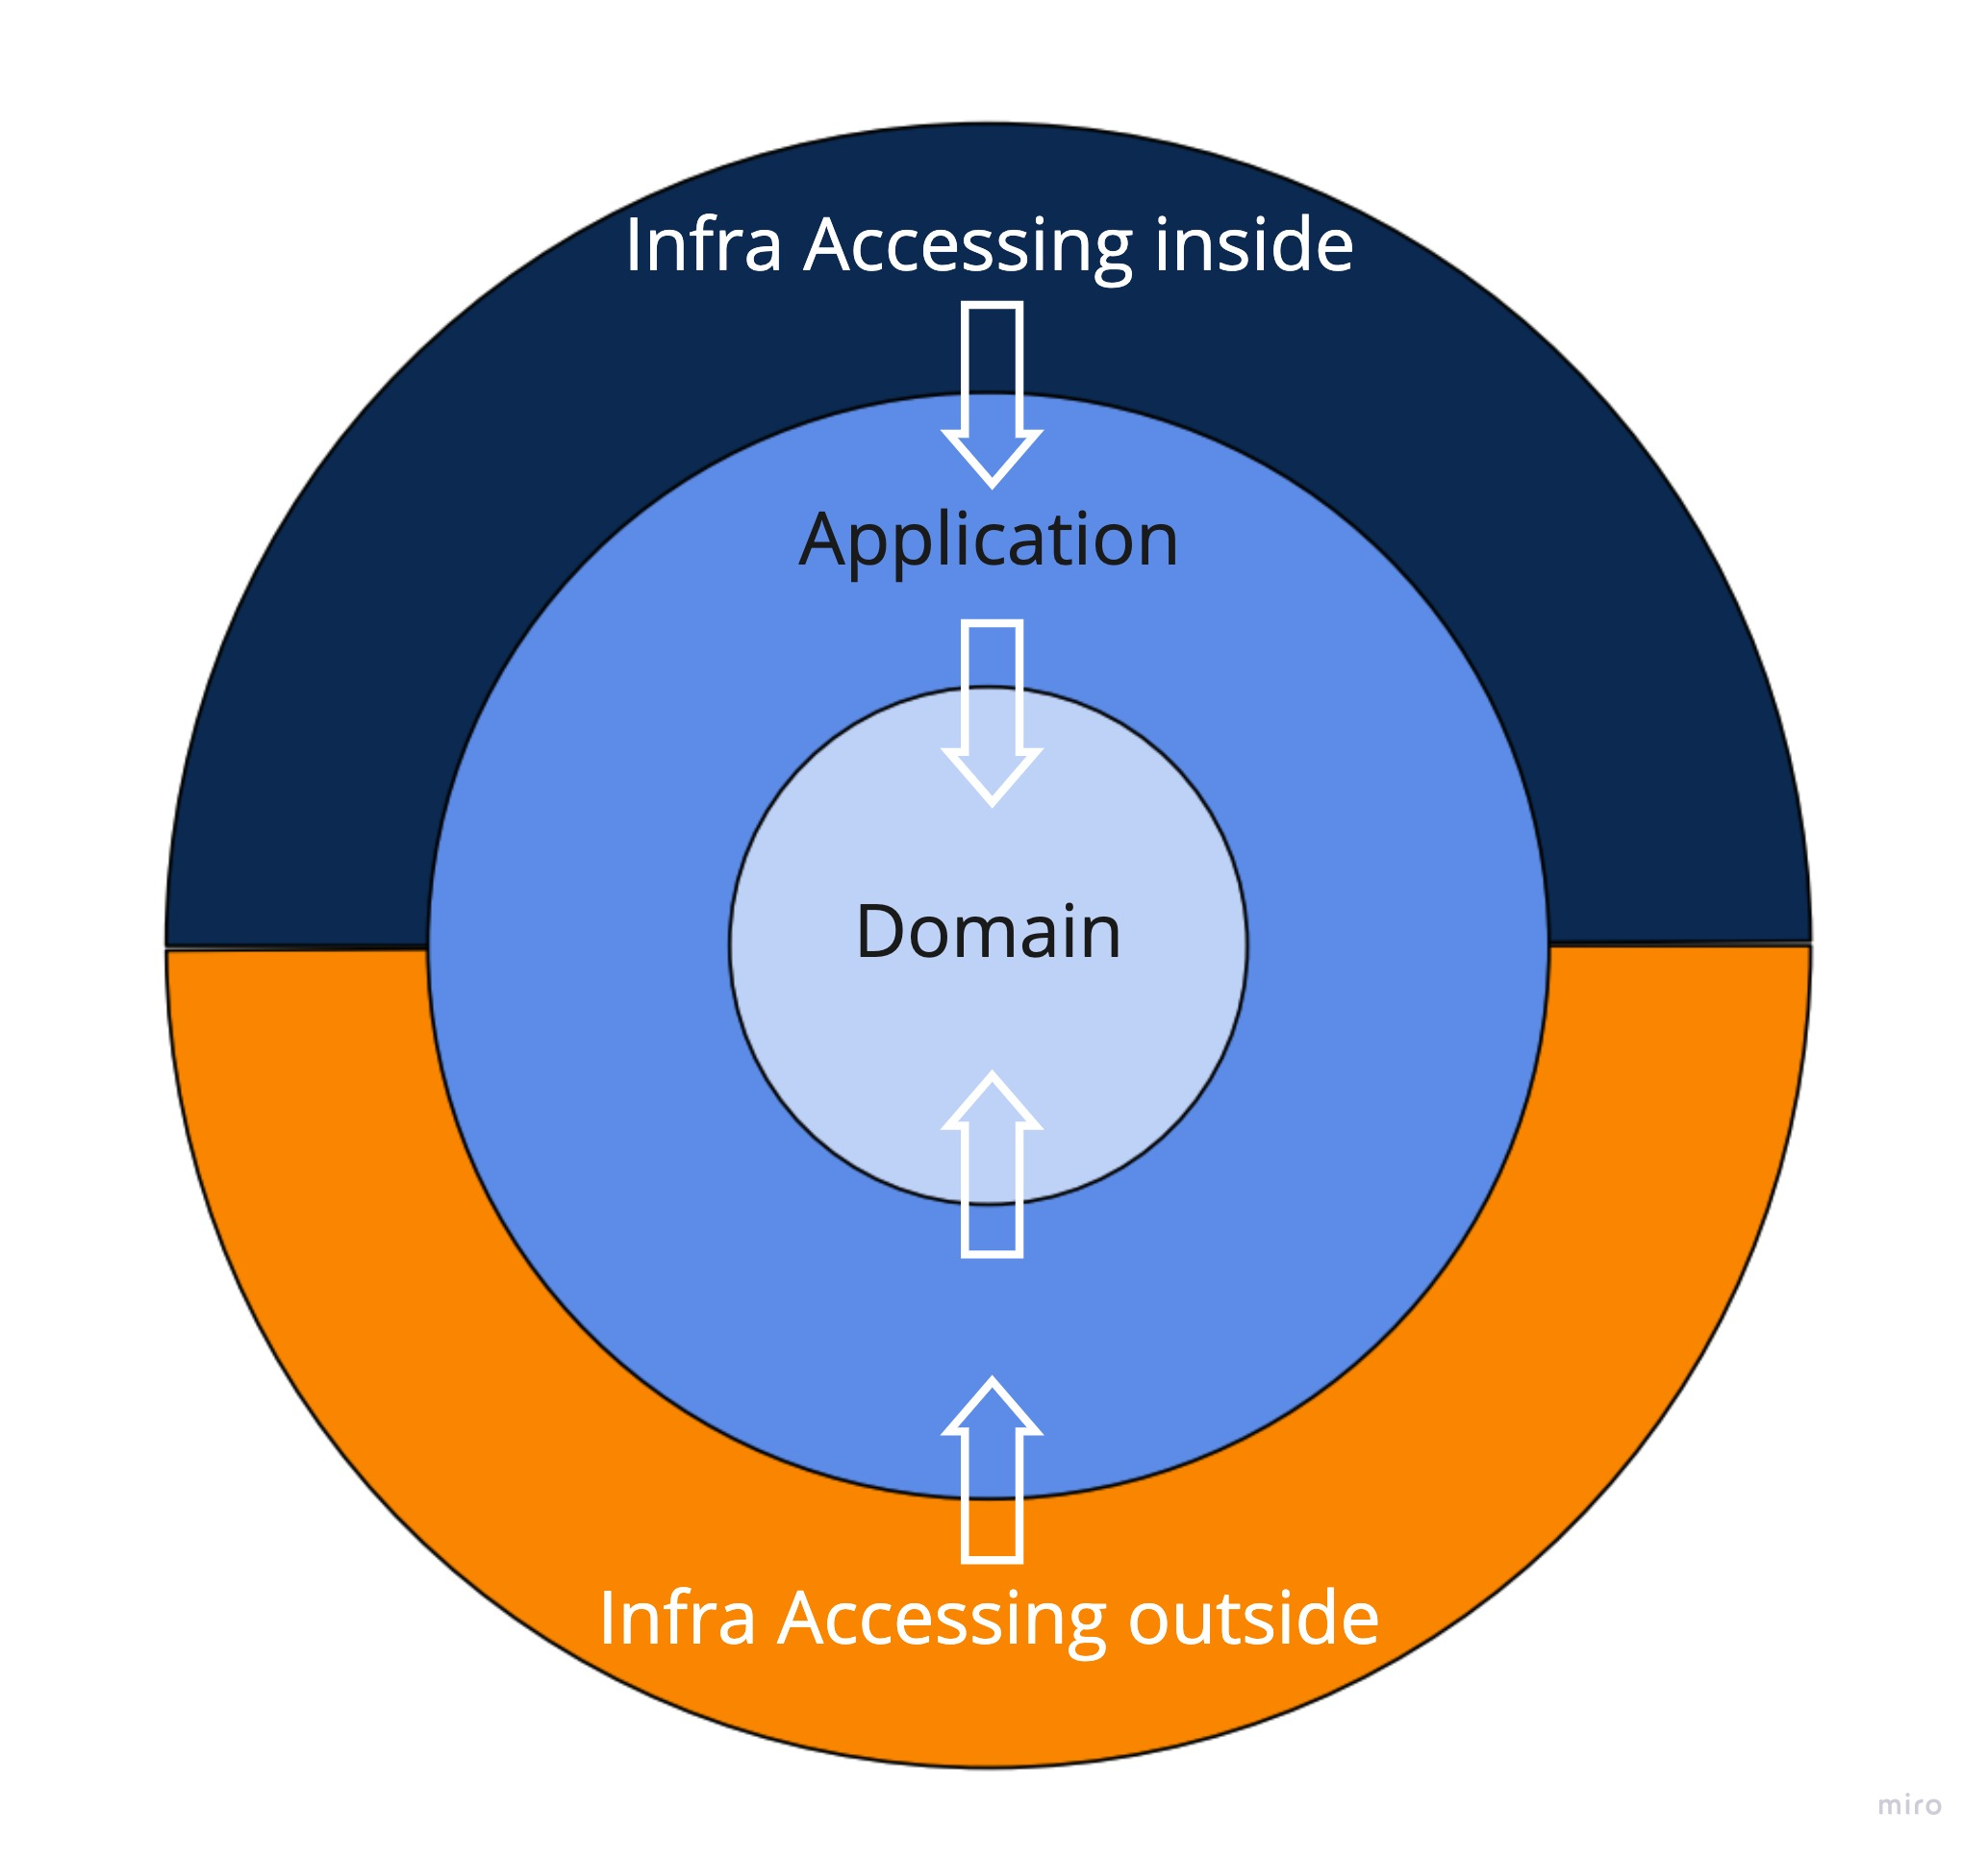
\includegraphics[height=0.3\textheight]{./part/Proyecto_ejecutivo/memoria_descriptiva/infoPreviaAntecedentes/img/PFM - Layer}
    \caption{Arquitectura de capas}\label{fig:layers}
\end{figure}

\paragraph{CQRS}

Junto con el concepto de arquitectura hexagonal y el\textit{DDD} vamos a aplicar el paradigma de diseño conocido como \gls{CQRS} (Command Query Responsibility Segregation). Es una técnica de diseño de arquitectura de software que separa la lógica de escritura (comandos) de la lógica de lectura (consultas) en sistemas de información. La idea es que las operaciones de escritura (comandos) y las operaciones de lectura (consultas) se manejen por separado, ya que tienen necesidades y características distintas. Mientras que las operaciones de escritura son responsables de modificar el estado de la aplicación, las operaciones de lectura son responsables de devolver información sobre ese estado sin modificarlo. Al separar estas dos responsabilidades, se pueden optimizar las operaciones de lectura para que sean más rápidas y escalables. Además, se puede diseñar una arquitectura de software más flexible, permitiendo una mayor adaptabilidad y evolución del sistema a medida que cambian los requisitos de la aplicación.

El resumen hasta ahora es que el diseño sigue una arquitectura hexagonal, con un enfoque\textit{DDD} en el dominio y un enfoque CQRS en los casos de uso. Es decir se diseñará un dominio rico y con un UL y se accederá a su funcionalidad a través de casos de uso que sigan el criterio de ser comandos y consultas.

\paragraph{Mapping}

El último detalle a explicar es cómo garantizar la separación efectiva de las capas en su uso de los elementos básicos con los que interactuan. Si un elemento de Infraestructura utiliza directamente una Entity de Dominio estaría saltando la capa de aplicación en su diagrama de dependencia. Bien es cierto que se mantendría la dependencia de fuera hacia adentro, pero se ha de tomar una decisión de hasta qué punto se quiere desacoplar una capa de otra. A esta decisión de diseño se le conoce como Estrategia de Mapping entre capas. Estrictamente cada capa requiere sus objetos de trabajo para estar desacoplada de las demás, pero como en todo aspecto de diseño está sometido a discusión acerca de seguir la teoría al pié de la letra y el pragmatismo de no verse envuelto en redundancias y sobredimensionar las soluciones.

En un extracto del libro Get Your Hands Dirty on Clean Architecture\cite{TomHombergs2019GYHD} podemos leer un extracto que es interesante rescatar ya que representa una conversación demasiado habitual entre compañeros de trabajo:

\textit{ The argument might have gone something like this:}

\begin{itemize}
    \item \textit{Pro-Mapping Developer:}
    \subitem  \textit{ If we don’t map between layers, we have to use the same model in both layers which means that the layers will be tightly coupled!}
    \item \textit{Contra-Mapping Developer:}
    \subitem \textit{ But if we do map between layers, we produce a lot of boilerplate code which is overkill for many use cases, since they’re only doing CRUD and have the same model across layers anyways!}
\end{itemize}
\textit{As is often the case in discussions like this, there’s truth to both sides of the argument. Let’s discuss some mapping strategies with their pros and cons and see if we can help those developers make a decision.}

Hay tantas estrategias como atajos dentro de este paradigma queramos asumir. Todo buen diseñador técnico debe saber tanto la teoría como los atajos que se pueden tomar. Evaluar los beneficios e inconvenientes y tomar una decisión con la que se ha de ser consecuente, y más importante en desarrollo, consistente. Esto quiere decir que una vez tomada una decisión debe ser una decisión en equipo que todos sigan. Es más eficiente un diseño imperfecto que sea consistente que un diseño perfecto en unos puntos e imperfecto en otros. Esto lleva al desorden a la hora de escribir código y complica la entrada de nuevos compañeros, el entendimiento del código existente con todas las consecuencias negativas que esto conlleva.

Los tipos de mapping que se documentan en este libro\cite{TomHombergs2019GYHD}:
\begin{itemize}
    \item The No Mapping Strategy~\cref{fig:nomapping}
    \item The Two-Way Mapping Strategy~\cref{fig:twowaymapping}
    \item The Full Mapping Strategy~\cref{fig:fullmapping}
    \item The One-Way Mapping Strategy~\cref{fig:onWaymapping}
\end{itemize}

Vamos a tomar diagramas del libro para entender cada estrategia. En todos los casos vemos simplificado el dominio a una única entidad, Account, y vemos como separa dicho dominio del acceso al caso de uso que envía dinero a una cuenta y del acceso a la infraestructura que guarda la información del envío de ese dinero.

\begin{figure}[H]
    \centering
    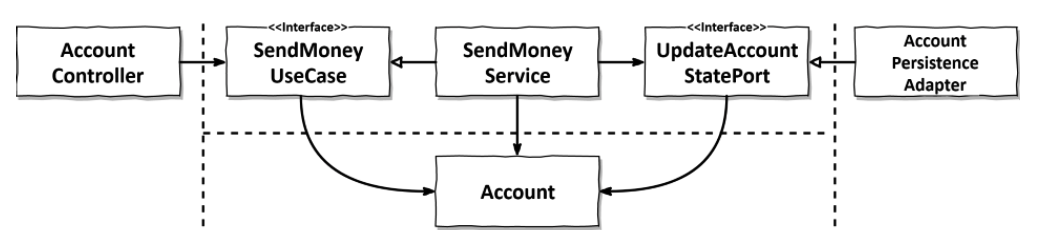
\includegraphics[height=0.1\textheight]{./part/Ejecucion/Seguimiento/CreateTaskUseCase/img/nomapping}
    \caption{No mapping strategy~\cite{TomHombergs2019GYHD}}\label{fig:nomapping}
\end{figure}

En la estrategia de No Mapping podemos ver en la figura~\cref{fig:nomapping} que tanto aplicación como Infraestructura dependen de Dominio. Esto evita todo código redundante, los \gls{DTO} (Data Transfer Object), pero resta flexibilidad. Si por detalles técnicos de una infraestructura concreta se requiere más o menos parámetros que los definidos en el Dominio o se deben guardar en otro formato que los definidos en Dominio enfrentaremos un problema.

\begin{figure}[H]
    \centering
    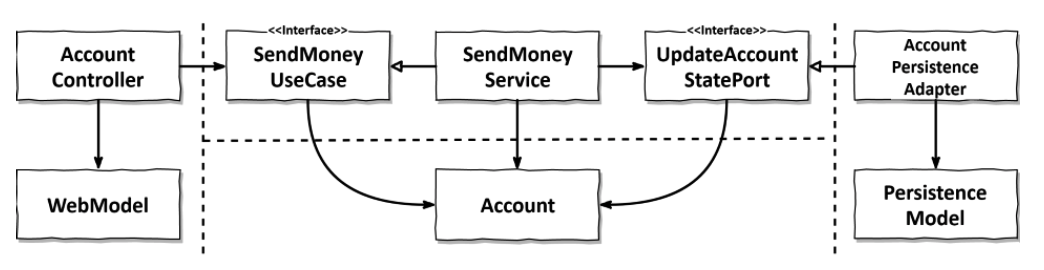
\includegraphics[height=0.1\textheight]{./part/Ejecucion/Seguimiento/CreateTaskUseCase/img/twowaymapping}
    \caption{Two way mapping strategy~\cite{TomHombergs2019GYHD}}\label{fig:twowaymapping}
\end{figure}

En la estrategia de Two-Way Mapping Strategy~\cref{fig:twowaymapping} nos deshacemos de este problema y creamos un modelo DTO que sirva para transportar la información de una capa a otra necesaria para conformar la Entidad. De esta forma puede evolucionar por separado. Seguimos contemplando ese posible problema problema entre la Aplicación, los casos de uso, y el Dominio. Además tenemos que escribir más código para crear las entidades a través de los DTO y viceversa.

\begin{figure}[H]
    \centering
    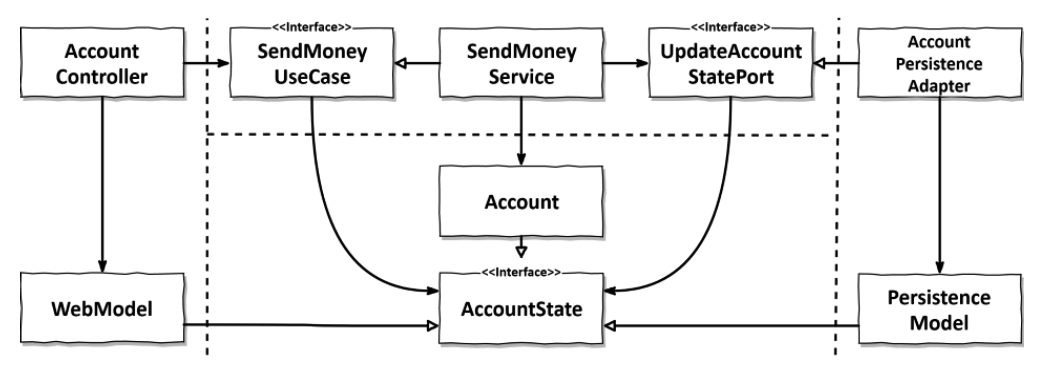
\includegraphics[height=0.1\textheight]{./part/Ejecucion/Seguimiento/CreateTaskUseCase/img/onWaymapping}
    \caption{One way mapping strategy~\cite{TomHombergs2019GYHD}}\label{fig:onWaymapping}
\end{figure}

En la figura de The One-Way Mapping Strategy~\cref{fig:onWaymapping} vemos que creamos una interfaz para la Entidad y hacemos depender de nuevo todas las capas de dicha interfaz. Se encuentran las capas más separadas y preparadas para el caso en el que se enfrente la necesidad de tener que crear distintas implementaciones aunque no se creen en un primer momento.

\begin{figure}[H]
    \centering
    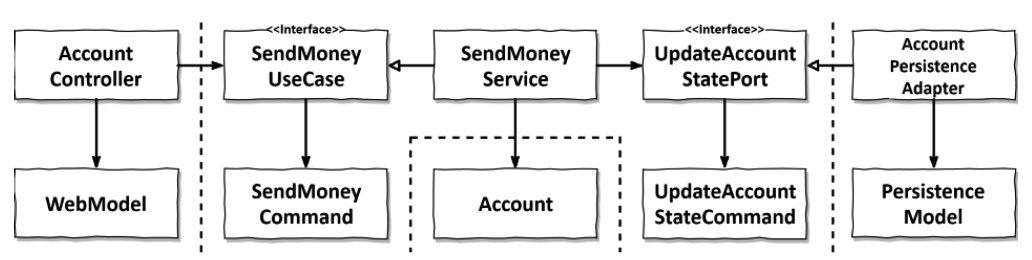
\includegraphics[height=0.1\textheight]{./part/Ejecucion/Seguimiento/CreateTaskUseCase/img/fullmapping}
    \caption{Full mapping strategy~\cite{TomHombergs2019GYHD}}\label{fig:fullmapping}
\end{figure}

En la figura de The Full Mapping Strategy~\cref{fig:twowaymapping} se opta por crear DTOs entre todas las capas. Es la solución más pura, pero el tradeoff es evidente: la cantidad de código a realizar es considerable y tiene que estar justificada con una necesidad de aislar hasta este punto.

No hay una regla de oro para elegir una estratégia que valga para todos los casos. Se reitera que debe ser una decisión de equipo, seguir la decisión todos y reevaluar con cada inconveniente que enfrente la decisión si se tiene que cambiar la estrategia.

Se puede ver el primer ejemplo en el un proyecto de ejecución que intentara resolver todas las decisiones y describir al detalle la solución a desarrollar no aportaría valor. Tomar una decisión de este tipo y documentarla, carece de utilidad porque no disponemos de información suficiente para tomar la decisión. Cuando nos enfrentamos al código es cuando podemos ver qué estrategia encaja mejor en nuestro caso.

\paragraph{Testing}
    \input{./part/Proyecto_ejecutivo/memoria_descriptiva/prestaciones/testing.tex}

\paragraph{Docker}

Docker es el sistema de gestión de contenedores más utilizado en la industria a día de hoy. Según la misma página oficial de Docker un contendor se define como: "A container is a standard unit of software that packages up code and all its dependencies so the application runs quickly and reliably from one computing environment to another. A Docker container image is a lightweight, standalone, executable package of software that includes everything needed to run an application: code, runtime, system tools, system libraries and settings."~\cite{docker}

El sistema se basa en la definición de imágenes que no son más que las instrucciones para la construcción de esos contenedores mediante el sistema de Docker Engine. Difieren de las máquinas virtuales tal y como se muestra en la comparativa~\cref{fig:Docker vs VM}.

Esto permite correr multiples aplicaciones con multiples requerimientos en cualquier máquina sin tener que instalar dichas dependencias de forma local, evitando incompatibilidades e interacciones no deseadas. Permite ofrecer entregables consistentes a los clientes de forma que el software y todo aquello que necesita para ejecutarse se entregan de forma conjunta, evitando problemas de instalación.

\begin{figure}[H]
    \centering
    \includegraphics[height=0.3\textheight]{./part/Proyecto_ejecutivo/memoria_descriptiva/prestaciones/docker/img/dockerVsVM}
    \caption{Docker vs VM.\cite{docker}}\label{fig:Docker vs VM}
\end{figure}

Las claves de Docker se basan en:
\begin{itemize}
    \item permite trabajar en el desarrollo de distintos proyectos con distintos requerimientos en una misma máquina sin la complejidad de mantener las dependencias de cada proyecto. O trasladarse a otra máquina y seguir trabajando de forma rápida al no tener que ponerse a instalar dichas dependencias de nuevo
    \item permite trabajar en equipo ya que cada cambio en las dependencias queda expresado en los cambios que se realizan de las imagenes de los contenedores que están disponibles para todo el equipo
    \item permite configurar el sistema para desarrollar o para producción de forma consistente con sus distintas diferencias en las dependencias necesarias, evitando problemas en el cambio de entorno de desarrollo y producción
\end{itemize}
\subsubsection{Descripción del proyecto}
    
\begin{figure}[H]
    \centering
    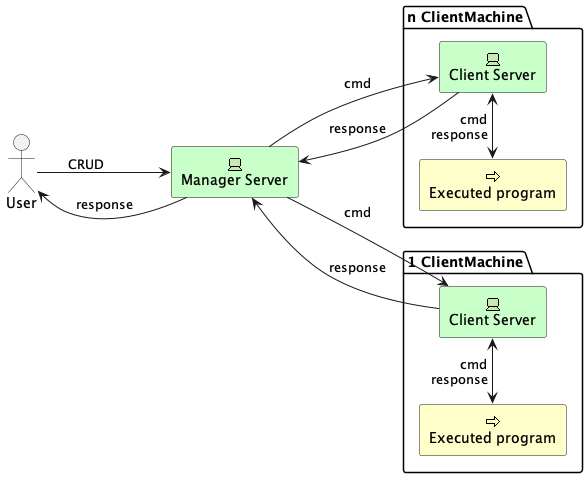
\includegraphics[height=0.4\textheight]{part/memoria_descriptiva/systemConcept}
    \caption[]{}\label{fig:systemConcept}
\end{figure}

Los componentes de esta solucion seran:
\begin{itemize}
    \item el manager server que guardará las tareas, las ejecutará y guardará el resultado.
    \item el client server que recepcionará las llamadas del manager con el comando y las ejecutará en el servidor cliente devolviendo los resultados al manager
    \item el programa a ejecutar. En nuestro caso haremos pruebas con varios ejecutables básicos, pero habrá un programa de control PID par aun motor de corriente continua
\end{itemize}

Se puede ver un diagrama conceptual del sistema en la figura~\ref{fig:systemConcept}. Vamos a proceder a describir cada uno de los programas de forma detallada. Esta descripción estará compuesta de los siguientes elementos:

\begin{itemize}
    \item diagrama de los componentes con los elementos con los que interacciona
    \item diagrama de objetos de sus elementos de dominio
    \item casos de uso: descripción y diagrama
    \item diagramas de procesos
    \item estructura de carpeta para la organización del código
\end{itemize}

\paragraph{Manager Server}

\begin{figure}[H]
    \centering
    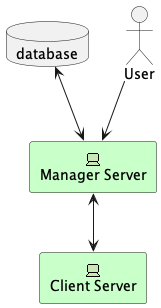
\includegraphics[height=0.4\textheight]{part/memoria_descriptiva/managerServerConcept}
    \caption[Diagrama componentes]{}\label{fig:managerServerConcept}
\end{figure}

\subparagraph{Dominio}

En el diagrama UML~\ref{fig:managerDomain} vemos que el dominio de Manager se compone de dos modulos: uno para las tareas y otro para los resultados. Vamos a ir explicando uno por uno:

\begin{itemize}
    \item Core
        \begin{itemize}
        \item Id todos los ids extenderan de este id, contiene un uuid, no sabemos que paquete usaremos para generarlos, es una de las pocas dependencias externas que vamos a tener dentro del dominio y queremo encapsularla lo máximo posible por si hubera que cambiarla. Además de esta forma los ids de las entities no se confunden en su tipo. si por ejemplo buscas una task mediante un id que corresponde a un result, si fueran del mismo tipo daría lugar a confusión porque no lo encontraríamos pero no nos advertiría de nuestro error
        \item Event todos los eventos del sistema extenderan del evento este
    \end{itemize}
    \item Task
        \begin{itemize}
        \item TaskId
        \item Host: es un Value Object compuesto por el valor del host, es un string pero el Value Object garantiza que es un valor válido, si no devuelve un error
        \item Port: es un Value Object compuesto por el valor del puerto, es un string pero el Value Object garantiza que es un valor válido, si no devuelve un error
        \item CommunicationMode: es un enum para expresar esa tarea de las formas de comunicación posibles que hay entre dos servidores cual sera la utilizada
            \begin{itemize}
                \item UNARY
                \item SERVER\_STREAM
                \item CLIENT\_STREAM
                \item BIDIRECTIONAL
            \end{itemize}
        \item ExecutionMode: es un enum
            \begin{itemize}
                \item MANUAL
                \item AUTOMATIC
            \end{itemize}
        \item Status: es un enum
            \begin{itemize}
                \item PENDING
                \item RUNNING
                \item SUCCESSFUL
                \item FAILED
            \end{itemize}
    \end{itemize}
    \item Step: cada tarea puede componerse en distintos pasos. Por ejemplo queremos poder poner en marcha el motor durante 15 segudos y luego llevarlo a una posición de inicio
    \begin{itemize}
      \item StepId
      \item sentence: será un string de contenido libre que el servidor cliente ejecutará en su sistema, dependerá de él tener instalado dicho programa y corroborar que la sintaxis es la correcta
    \end{itemize}
    \item TaskCreatedEvent. Cuando se cree una tarea se emitirá un evento, habrá un manejador de eventos que actuará en consecuencia. Si es una tarea automatizada y el loop de ejecución está parado lo pondrá en marcha.
    \item TaskModifiedEvent: si una tarea es modificada se emitirá un evento, habrá un manejador de eventos que actuará en consecuencia. Si la tarea vuelve a ser puesta a pending, es automatizada y el loop de ejecución está parado lo pondrá en marcha
    \item TaskDeletedEvent: si una tarea es modificada se emitirá un evento, habrá un manejador de eventos que actuará en consecuencia.
\end{itemize}

\begin{figure}[H]
    \centering
    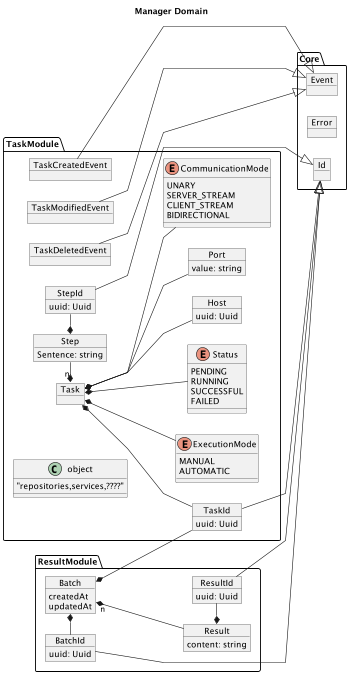
\includegraphics[height=0.4\textheight]{part/memoria_descriptiva/managerDomain}
    \caption[Diagrama de objetos de dominio]{}\label{fig:managerDomain}
\end{figure}



\subparagraph{casos de uso}

Vamos a describir los casos de uso que podrán ejecutarse en el programa manager

\textbf{crear tarea}

\begin{figure}[H]
    \centering
    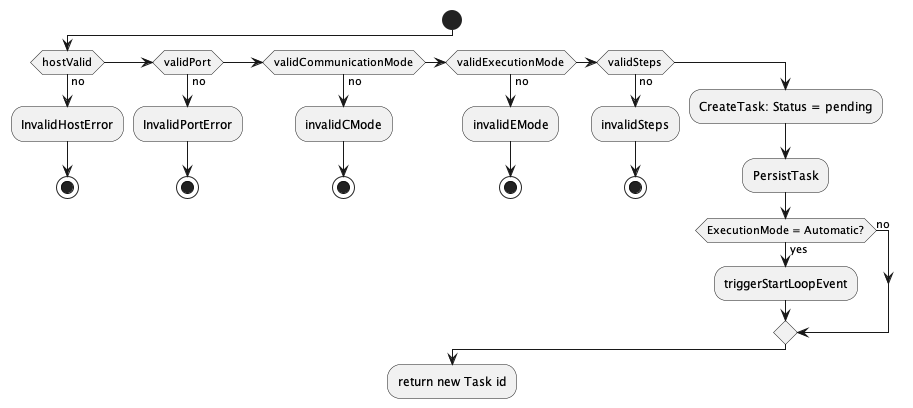
\includegraphics[height=0.3\textheight]{part/memoria_descriptiva/createTaskUseCase}
    \caption[Diagrama de objetos de dominio]{}\label{fig:createTaskUseCase}
\end{figure}

\textbf{obtener tarea}

\begin{figure}[H]
    \centering
    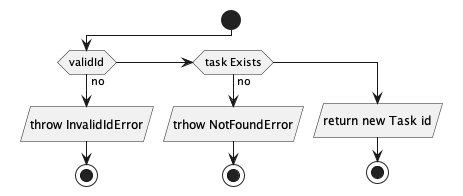
\includegraphics[height=0.3\textheight]{part/memoria_descriptiva/getTaskUseCase}
    \caption[Diagrama de objetos de dominio]{}\label{fig:getTaskUseCase}
\end{figure}

\textbf{listar tareas}

Uno de los puntos más amplios en una API CRUD es el filtrado de datos. No entra dentro del ámbito de este proyecto crear un sistema de filtrado que incluya la paginación. En este caso habría que crear una nomenclatura de filtros de cara al usuario y un sistema que los procese, devolviendo error ante un filtro erroneo o el listado de tareas que responda a dicho filtro. En nuestro caso devolveremos todas las tareas.

\textbf{actualizar tareas}

\begin{figure}[H]
    \centering
    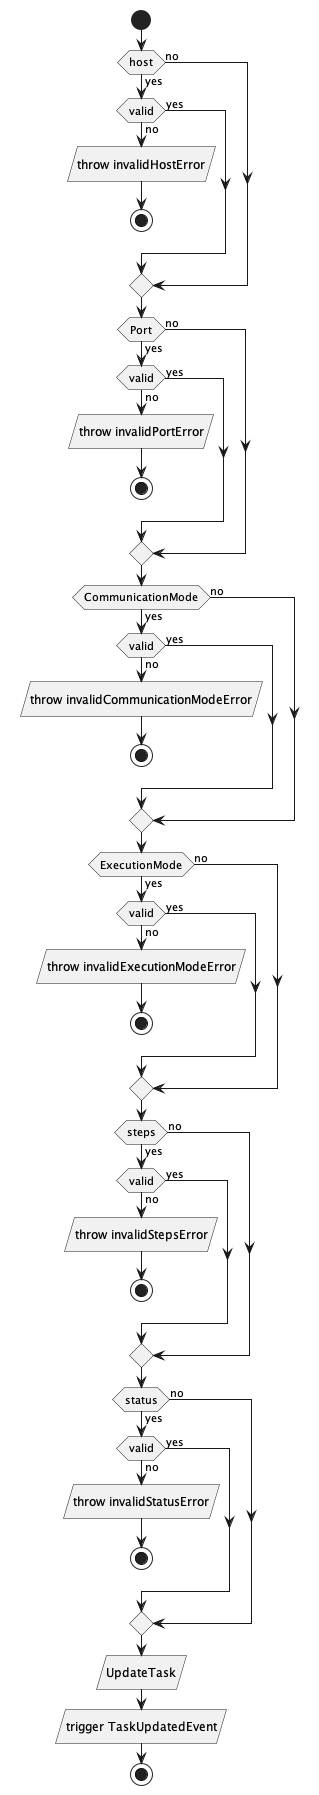
\includegraphics[height=0.5\textheight]{part/memoria_descriptiva/updateTaskUseCase}
    \caption[Diagrama de objetos de dominio]{}\label{fig:updateTaskUseCase}
\end{figure}

\textbf{eliminar tareas}

\begin{figure}[H]
    \centering
    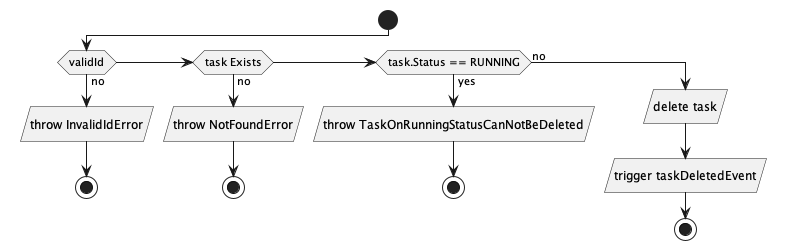
\includegraphics[height=0.2\textheight]{part/memoria_descriptiva/deleteTaskUseCase}
    \caption[Diagrama de objetos de dominio]{}\label{fig:deleteTaskUseCase}
\end{figure}

\subparagraph{estructura de carpetas}

Una de las partes mas importantes de un proyecto de software es que la estructura de carpetas hable sobre cómo está diseñado el software, sobre de qué va el software. qué es lo que hace y sobre que componentes interactua

\input{./part/memoria_descriptiva/folder_estructure_manager.tex}

Queda pendiente implementar aplicación e infraestructura. Cabe reseñar el apartado de aplicación loop handler. Vamos a detenernos en este concepto de aplicación que si merece la pena mención

\textbf{ejecutar loop de tareas automaticas}

handler que implementará aplicación porque el manual-automatic es muy complejo. al final habrá en este proceso muchos conceptos que descubriremos core de la aplicación y debieran ser dominio, pero como tenemos que descubrirlos vamos a implementarlos en aplicación haciendo uso de interfaces de infraestructura y de elementos de dominio. Si vemos claramente que algo puede convertirse en dominio lo introduciremos.


\paragraph{Client Server}

Hay que tener en cuenta que en este programa será casi todo infrestructura. ya que una vez recepcionado el comando mediante el RPC
solo quedará

En esta memoria descriptiva vamos a diseñar un sistema que tenga palabras clave para diferenciar un comando de pid y otro totalmente distinto. ya que si queremos ejecutar un simple comando de consola en el servidor cliente.

Las posibilidades son tantas como comandos haya instalados en el servidor cliente.

por ejemplo si el comando es ./runMyComand --arg=arg

como un típico comando de consola quedará a cargo del usuario de este progrmaa cliente implementar la interfaz

\paragraph{Control Program}

Casos de uso todas las funciones del engine y diseñarlo para que la infra sea a través de consola de comandos (preparando para que luego debido a la comunicación rpc devolver los datos sea muy complicado si lo dividimos en otro comando y decidimos absorver este dominio)

El sistema está pensado para que el programa a ejecutar sea de libre decisión del cliente. pero vamos a aprovechar la oportunidad para crear un programa de control y profundizar tanto en el uso del lenguaje como en los conocimientos relacionados con este master. En concreto el control automático. Uno do los programas que podrá ejecutar será un control PID.
\subsubsection{Prestaciones}
    \paragraph{Utilización}
    De cara al usuario cliente de este sistema dispondrá de:
    \begin{itemize}
        \item Un sistema para introducir y gestionar tareas para ejecutar en sistemas remotos de forma automática o manual
        \item Un programa cliente para ofrecer al público. Cualquier servidor con este programa instalado podrá recibir tareas desde el manager que se ejecutarán en su servidor de forma automática.
        \item Un programa de control pid para un microcontrolador para controlar un motor de corriente continua ejecutable desde consola. Por lo tanto cualquier cliente podrá instalarlo en su servidor y temporizar tareas sobre este programa.
    \end{itemize}

En un ejemplo básico de uso podríamos tener una puerta automática controlada por un microcontrolador y ejecutar la apertura desde el manager.

\paragraph{Seguridad y calidad}\label{par:testing}
    \input{./part/Proyecto_ejecutivo/memoria_descriptiva/prestaciones/testing.tex}
\paragraph{Robustez ante nuevos desarrollo}

Uno de los puntos más relevantes de un proyecto de software es garantizar la viabilidad en la continuidad del desarrollo futuro; ya sea por mantenimiento o adición de nuevas características.

Para esto hay que tener en cuenta que uno de los factores más limitantes es la acumulación de conocimiento acerca del sistema en los ténicos. Tener un sistema que evite tener que conocer todo el proyecto en profundidad para realizar cambios es crítico. Uno de estos puntos es la infraestructura. El hecho de instalar el sistema en su modo para el desarrollo es en sí un reto. Instalar dependencias y garantizar que todo está funcional.

Por ello es importante, no sólo la documentación, si herramientas que levanten el sistema de forma automatizada y generalizada para cualquier dispositivo. A nuestra disposición tenemos Docker~\cref{par:Docker}, scripts y archivos Makefile.

Dentro de esos contendores Docker dispondremos de todas las herramientas ya instaladas para manejar el sistema sin tener que instalarlas en nuestra propia máquina.

Para este proyecto necesitaremos garantizar:

\begin{itemize}
    \item versión fija de golang para compilar los programas
    \item versión fija de la las librerias
    \item versión fija de la base de datos
    \item configuración del protocolo de comunicación entre sistemas
\end{itemize}

tendremos un archivo Makefile en cada programa para:

\begin{itemize}
    \item interactuar con el sistema de contenedores docker~\cref{par:Docker}
    \item interactuar con el protocolo GRPC~\cref{subsubsec:communications}
    \item interactuar con la base de datos~\cref{par:mysql}
\end{itemize}





\subsection{Memoria constructiva}\label{subsec:memoria-constructiva}
	\subsubsection{lenguajes}
    

\textbf{Golang}


Uno de los puntos centrales de este trabajo es exponer el estado del arte en el uso de Golang para el entorno industrial. En dicho estudio se ha consultado distintos papers y publicaciones para extraer primeras conclusiones:

Uno de los puntos más importantes para el desarrollo de software industrial es los recursos consumidos una de las primeras conclusines extraidas de la eficiencia del uso de golang interaccionando con mysql, una de las combinaciones más comerciales concluye que: "... combination of Go and MySQL is superior regarding CPU utilization and memory usage, while Node.js and MySQL combination is superior regarding response time~\cite{Effendy20211955}".

Un estudio más centrado en el uso de recursos ante problemas de algorítmia con altos requerimientos, en particular la implementacion de un árbol de decisiones. ~\cite{Dymora20201} Donde encontramos un punto importante: golang vuelve a no dar ventajas, pero tampoco inconvenientes en materia de tiempos de ejecucion. pero si que pierde en uso de cpu claramente y empata en materia de uso de memoria para mas de 500K registros en este problema en particular. Aunque se admite que la optimización de dicho mecanismo para este problema. lo cual es posible. "Thus, the Go language garbage collector
supports programmers by automatically releasing their programs’ memory when it is no longer needed.
However, tracking and cleaning the memory requires additional resources such as CPU time. The effect
of this can be seen in Figure 5. Of course, the scope of optimizing"~\cite{Dymora20201}

lo que si nos permite extraer es una conclusion y es que para usos intensivos golang es una opción viable pero no da ventaja en este aspecto.

Esto se debe al mecanismo que le da una ventaja tan notoria en el uso menos intensivo: el garbage collector que le requiere un uso adicional de memoria y cpu para ejecuciones con un gran número de registros. Concluye este estudio diciendo: ". Go can be an
attractive alternative in the area of DevOps tools. It is attractive to build something small–medium
that works natively without using a lot of RAM and which runs fast with many things needed for
this task in the language itself"~\cite{Dymora20201}

\begin{figure}[H]
	\centering
	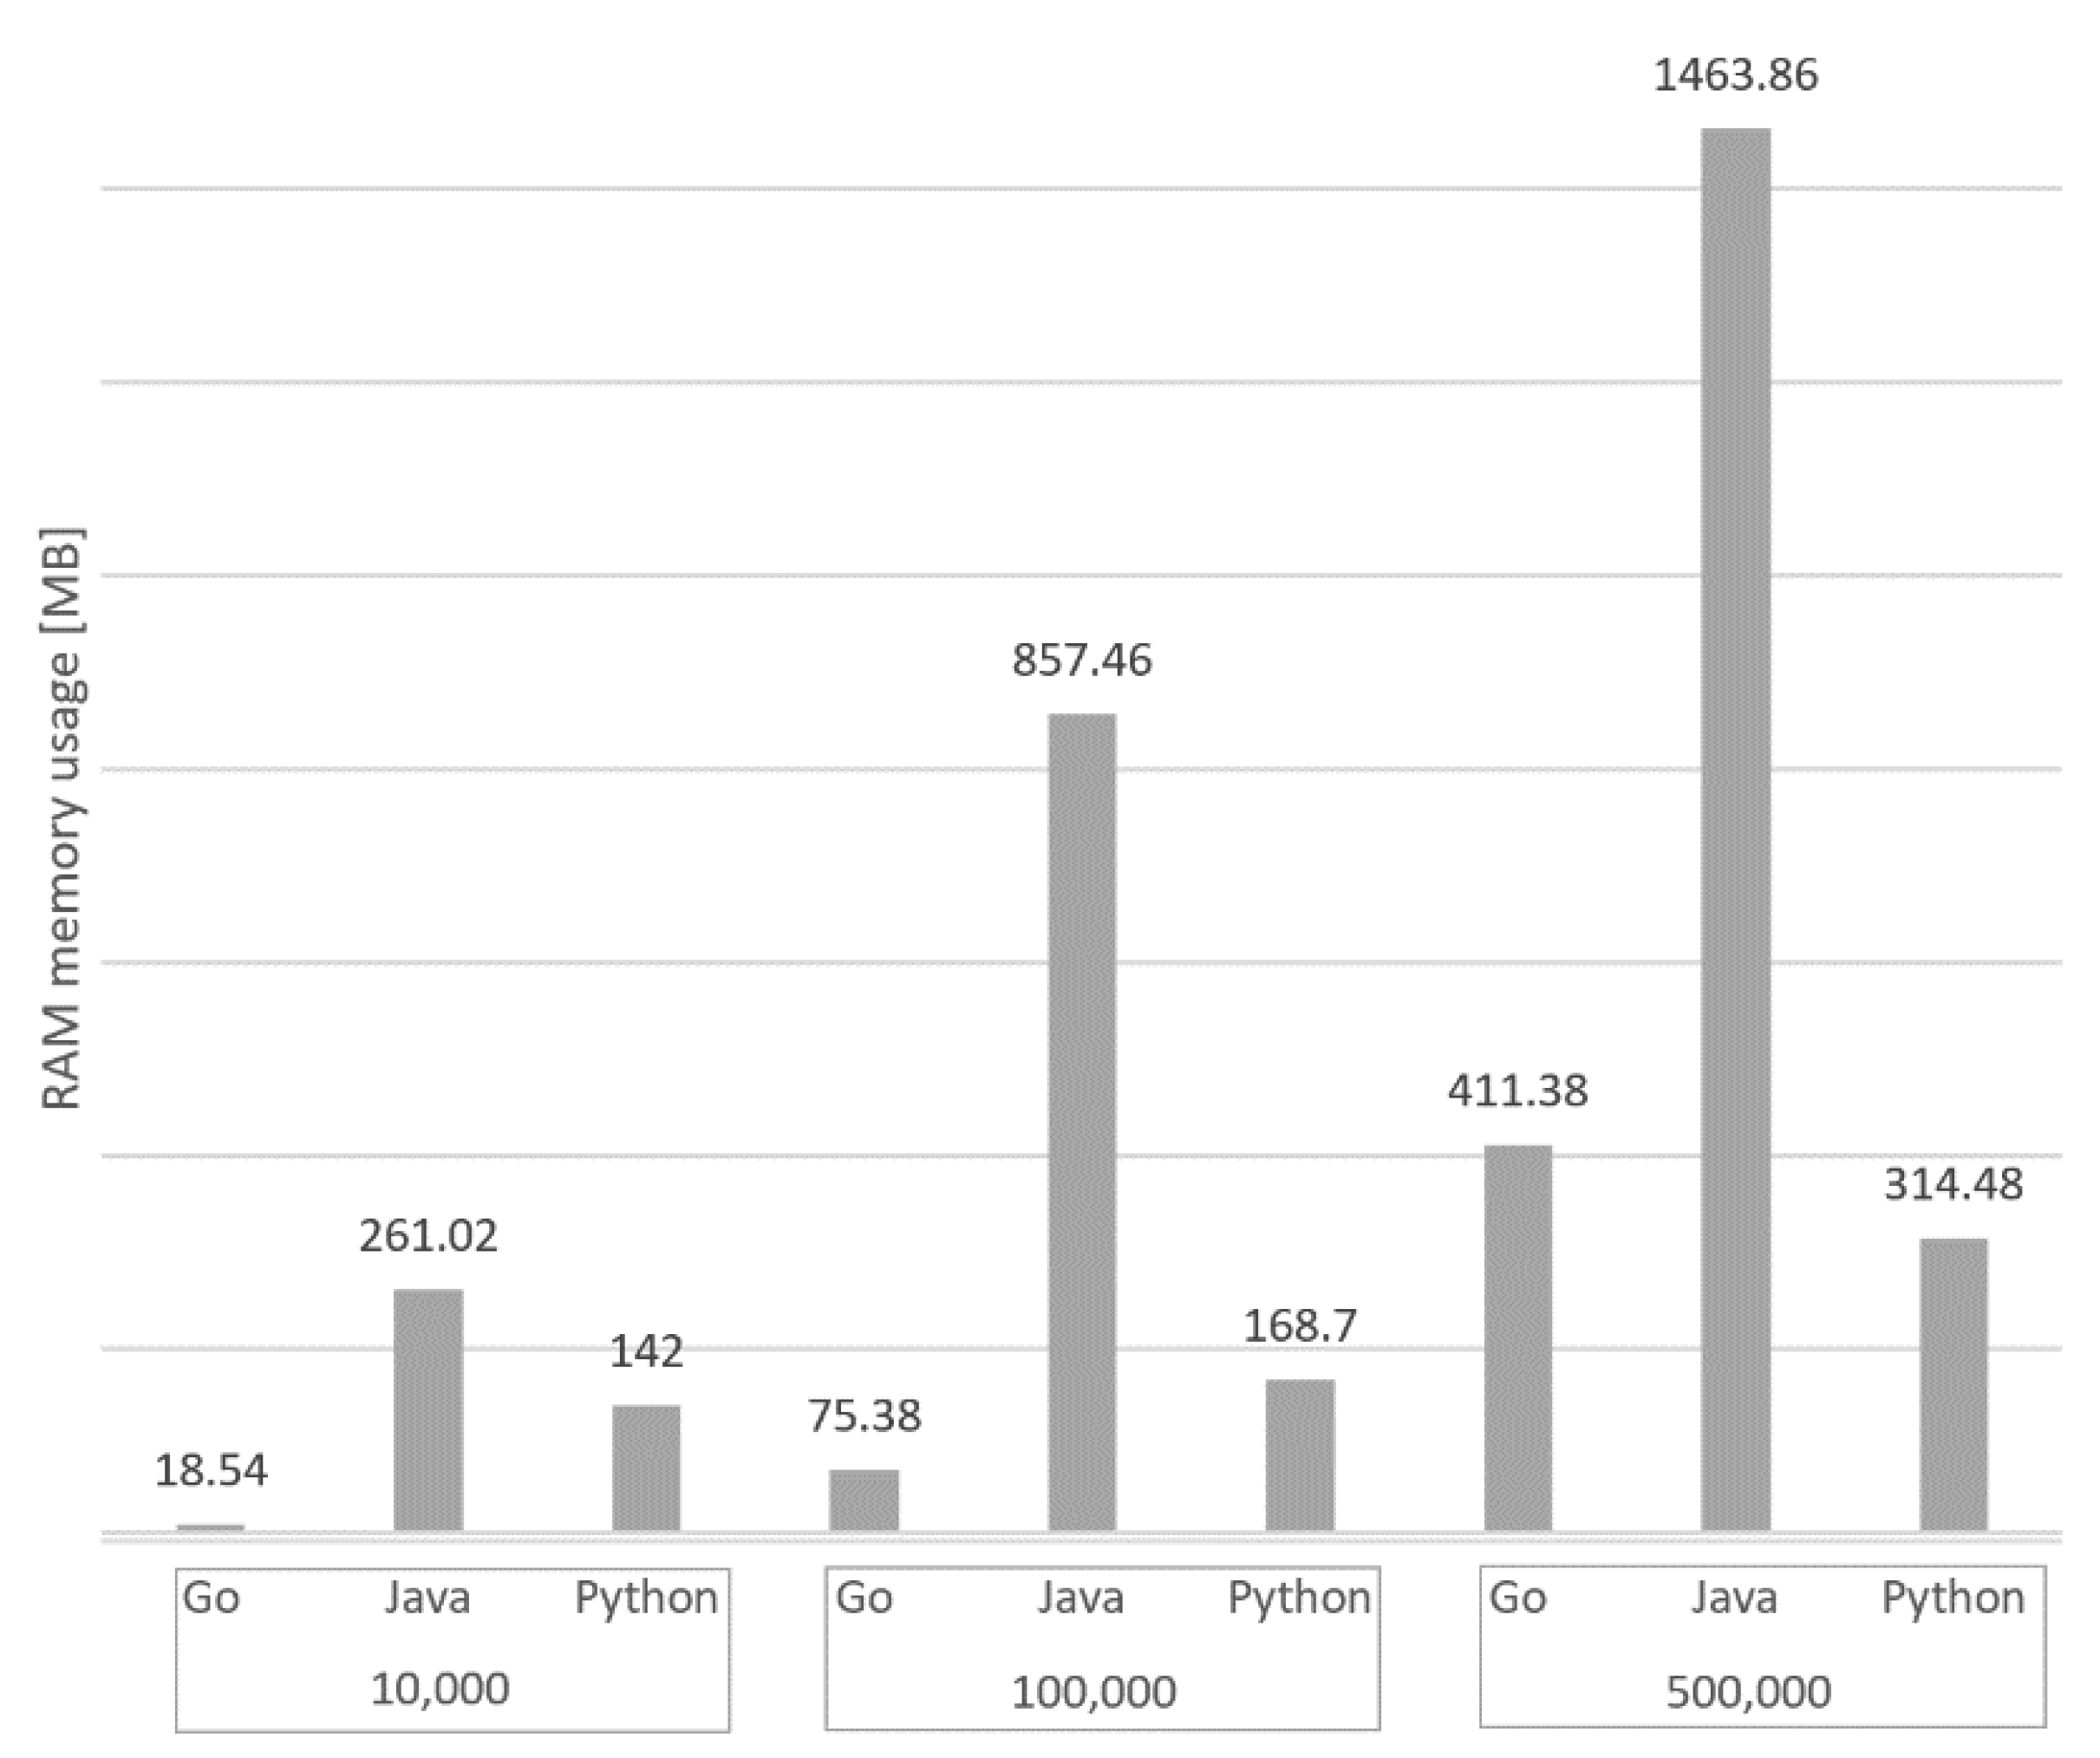
\includegraphics[height=0.3\textheight]{./part/Proyecto_ejecutivo/memoria_constructiva/golang/img/memory_usage}
	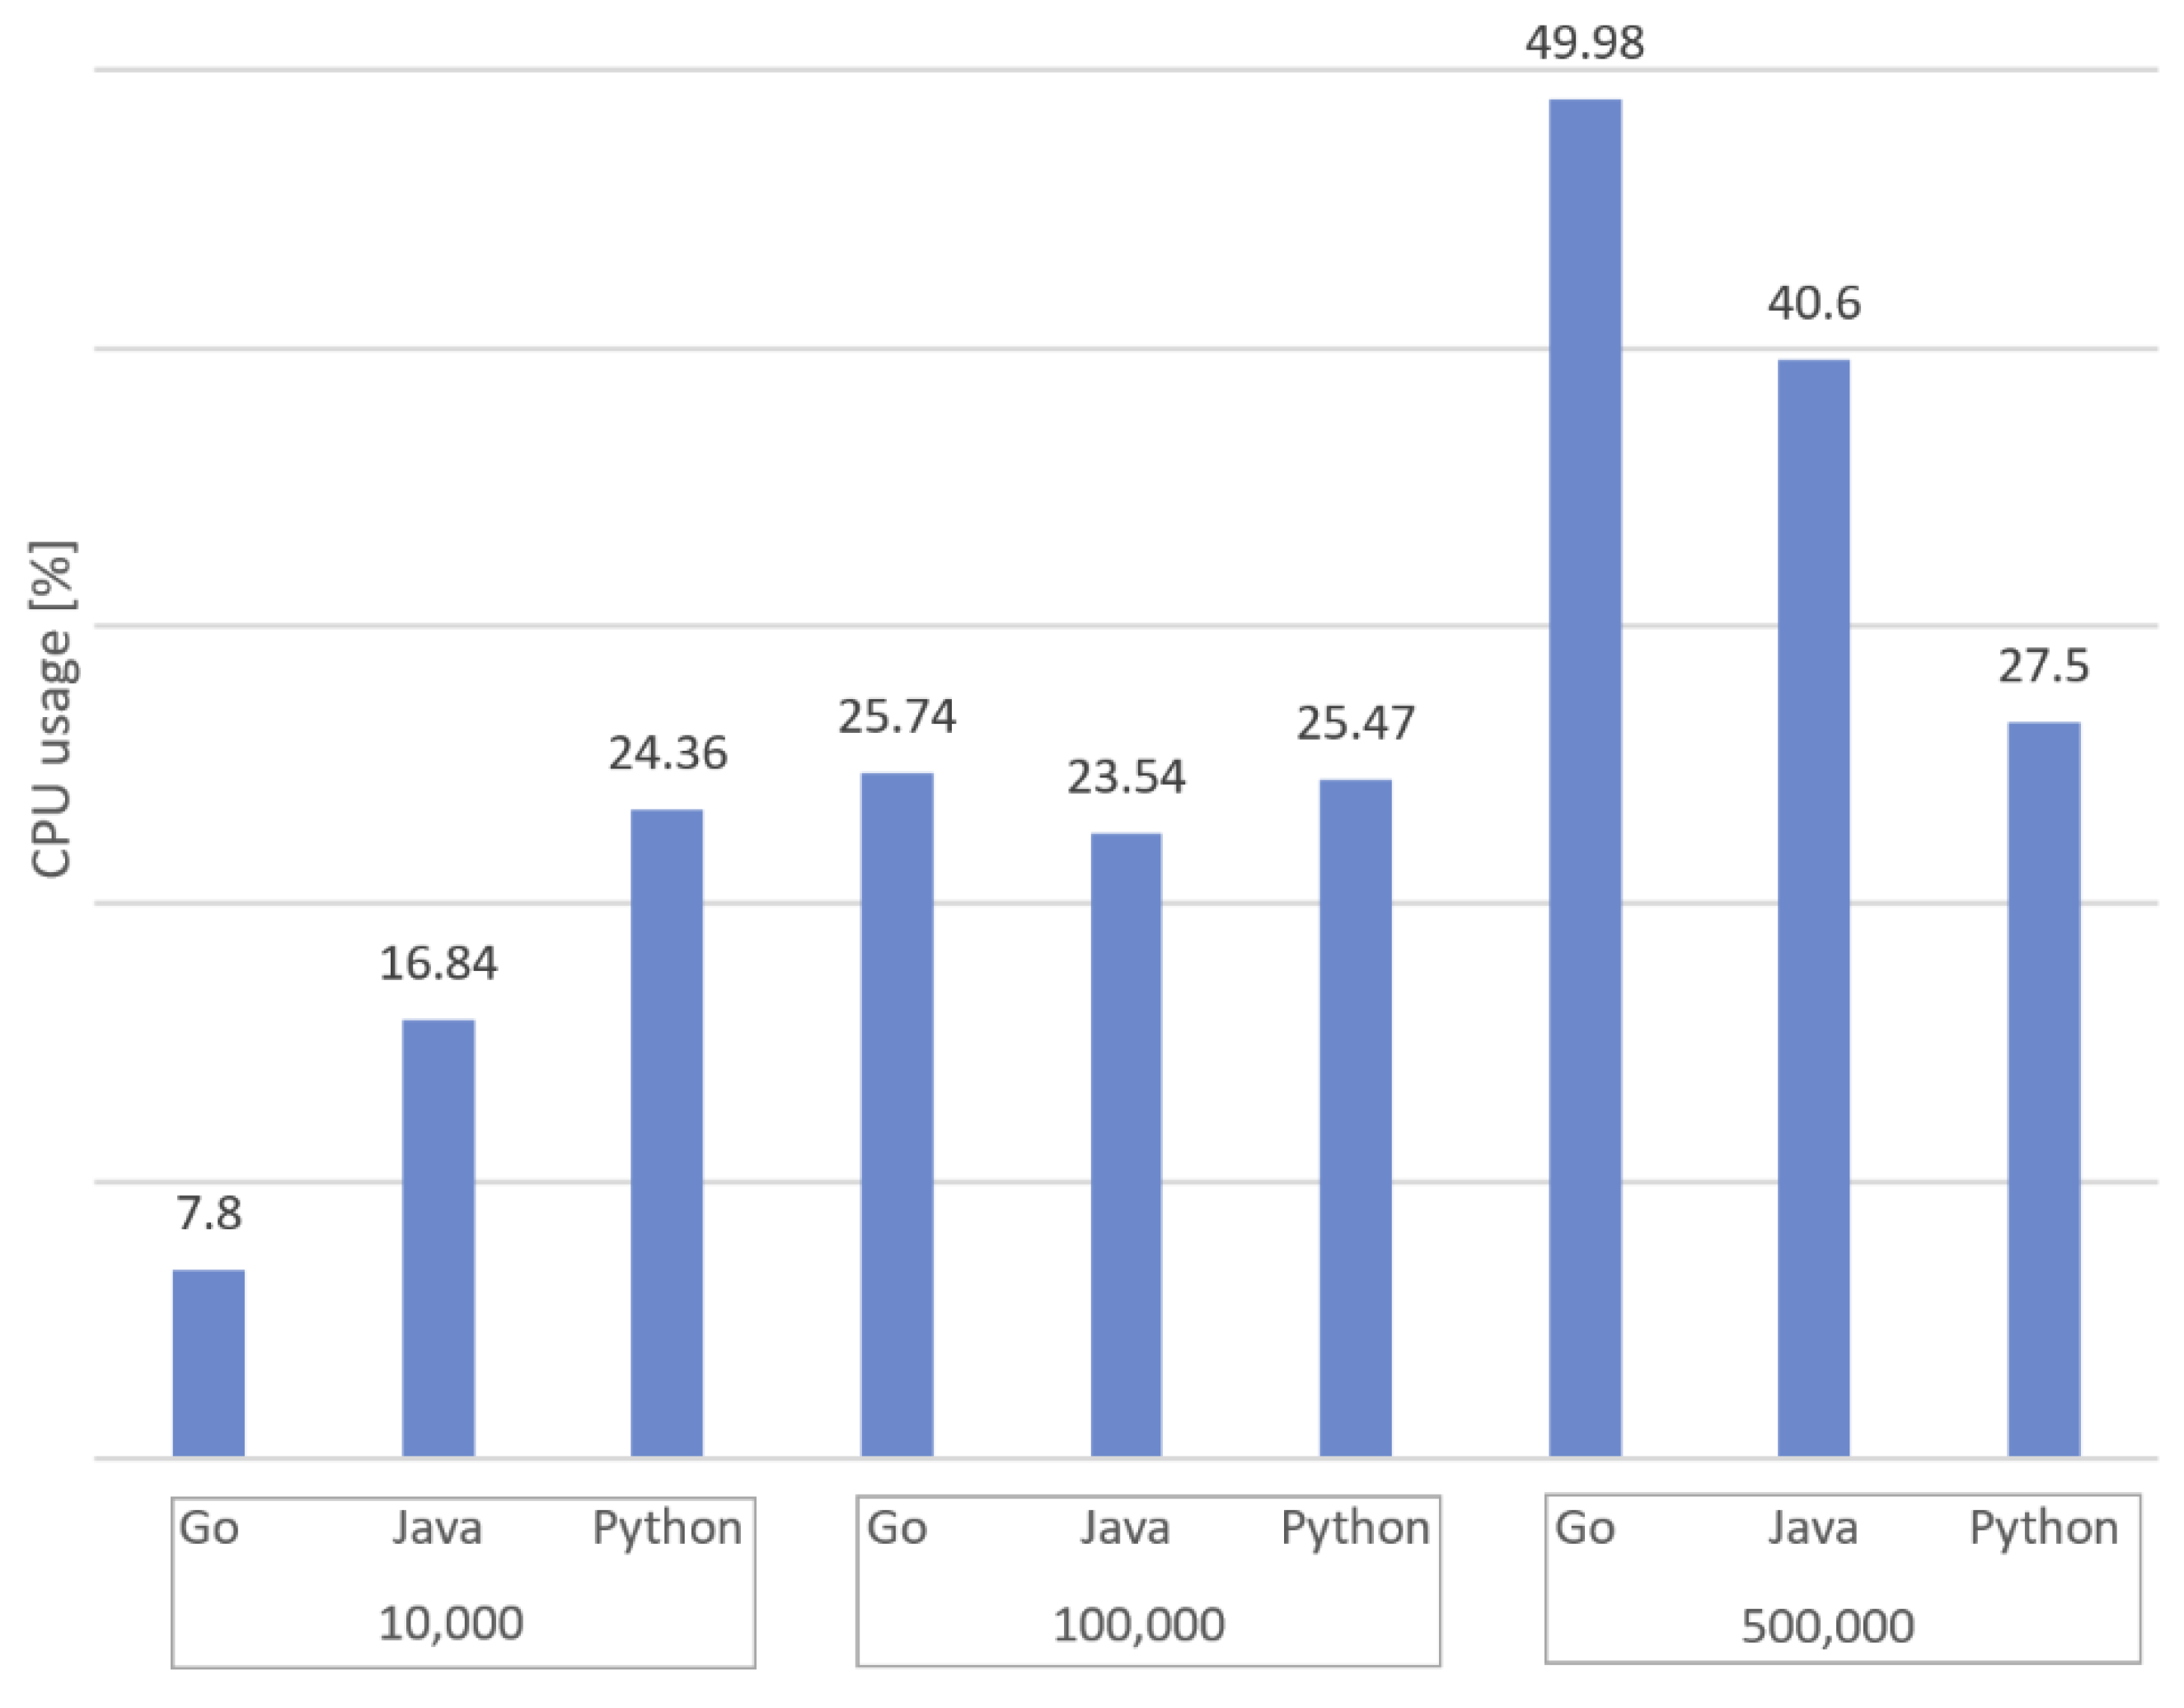
\includegraphics[height=0.3\textheight]{./part/Proyecto_ejecutivo/memoria_constructiva/golang/img/cpuUsage}
	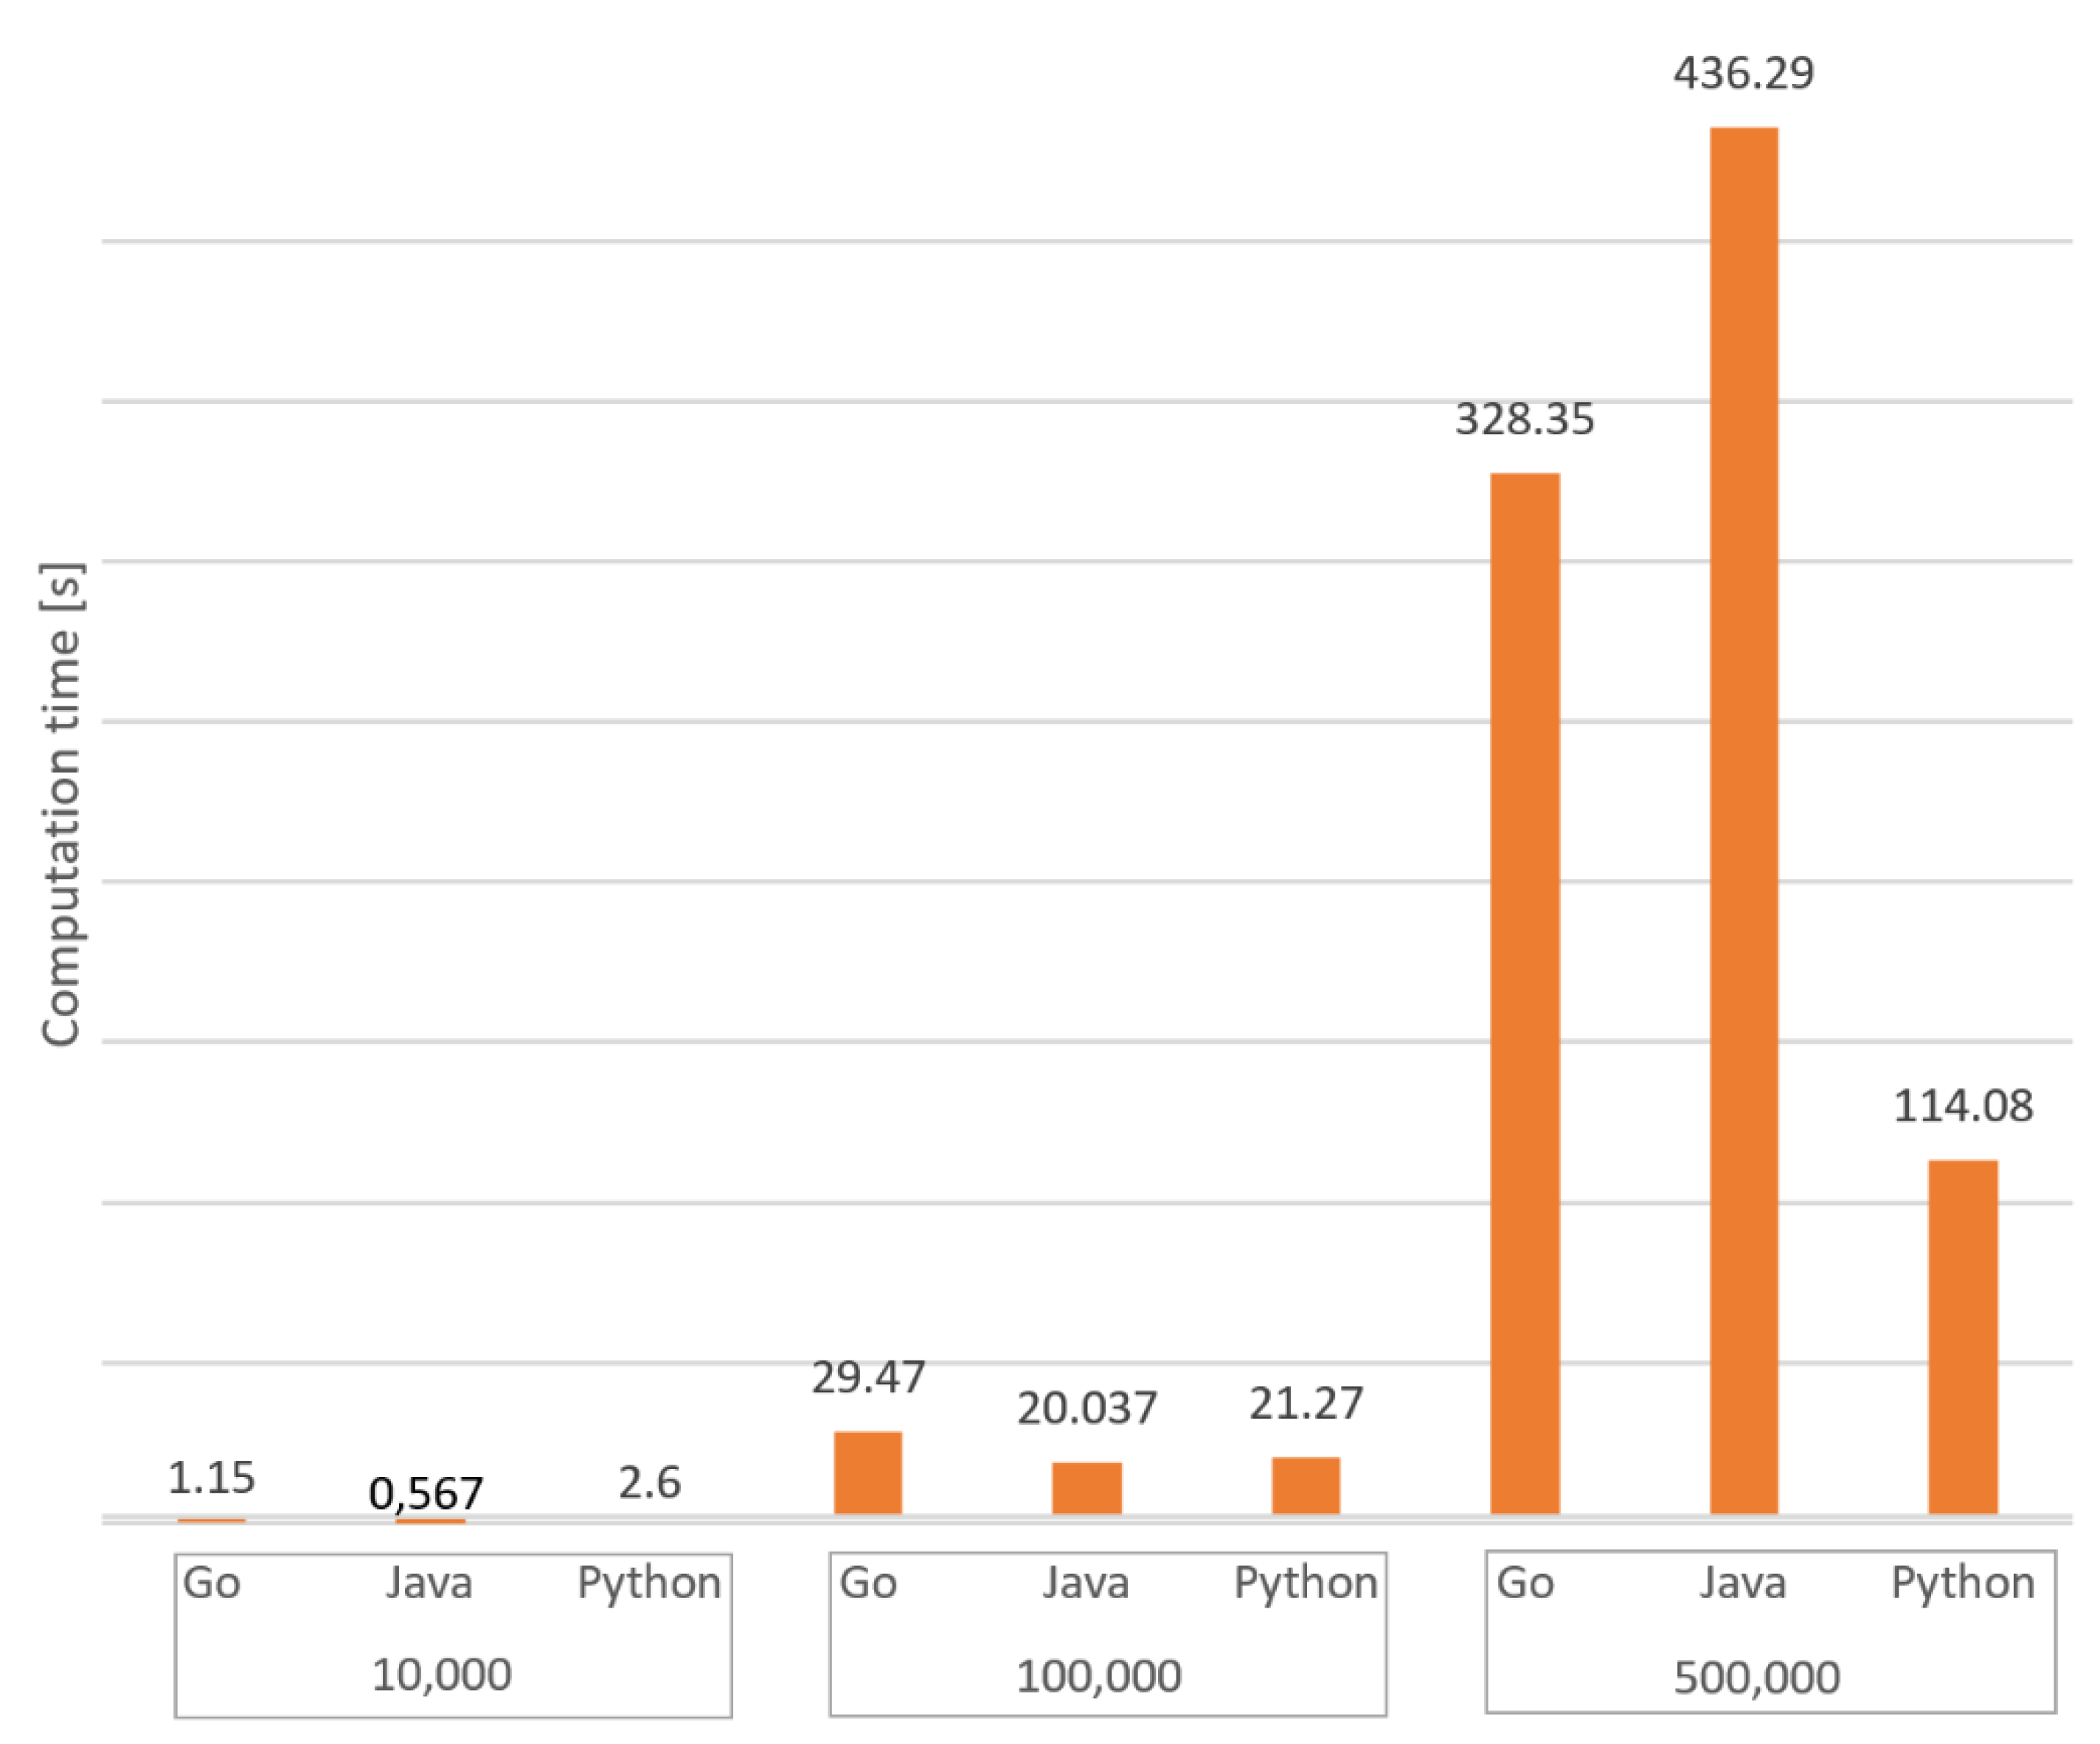
\includegraphics[height=0.3\textheight]{./part/Proyecto_ejecutivo/memoria_constructiva/golang/img/compTime}
	\caption[performance golang on algorithm]{performance golang on algorithm\cite{Dymora20201}}\label{fig:performance golang}
\end{figure}

El verdadero motivo para optar por golang como lenguaje para un software viene más de la mano de la facilidad de mantenimiendo, la rapidez de compilacion, el manejo fácil para la concurrencia y eficiente en el uso de recursos. Implementar mecanismos de memoria compartida para procesos concurrente es donde golang si optimiza recursos. Uno de los trabajadores de google que ha contribuido al ecosistema de go nos dice "Everyone knows and thinks about Google in terms of scale of users and scale of servers, but one thing that's not talked about as often is the scale of engineering effort."~\cite{Meyerson2014104+101}

Esto quiere decir que en la mayoría de las compañías el mayor coste no es el de infraestructura, si no el de ingeniería. Es un tradeoff muy importante el reducir el numero de horas dedicadas a mantener y desarrollar software que el hecho de optimizar el uso de máquinas. Si encima nos encontramos con un problema que no requiere de uso intensivo en cuestión algorítmica o tiempo de respuesta encontramos lo mejor de los dos: tenemos la ventaja de reducir los recuros necesarios de infraestructura y los de ingeniería. Si se diera el caso de que el software se enfrenta con el tiempo a problemas de escala siempre nos quedará la opción de aumentar las prestaciones de las máquinas utilizadas pero no tener problemas de aumento de costes de ingeniería

Es en la implementación de algoritmos que sacan ventaja de la concurrencia donde golang puede sacar ventaja respecto a otros lenguages como java o python ~\cite{Jenkins201714}

Estas son las principales conclusiones extraidas de la lectura de las publicaciones consultadas.
\cite{Effendy20211955}
\cite{Dymora20201}
\cite{Meyerson2014104+101}
\cite{Ray202110857}
\cite{Jenkins201714}
\cite{Ding2021321}
\cite{Taheri2021138}
\cite{NoAuthor2021179}
\cite{Dilley2019377}
\cite{Qiu2018}
\cite{Shoumik20181}
\cite{Mladenovic2018}
\cite{Benedict2017437}
\cite{Irawan2017}
\cite{Samaniego2017116}
\cite{Khaitan20152909}
\cite{Leokhin2015656}
\cite{Komendantskaya2014121}
\cite{Mittal2014292}
\cite{WhiteheadII2011209}
Nos permiten concluir que está justificado el uso en nuestro objetivo de diseñar un sistema de las carácteristicas de este proyecto con Golang.

Concluyo mencionando \cite{WhiteheadII2011209}"Despite the relatively young age of the programming language, we believe that Go helps
to fill an interesting niche in the field of programming languages. The unique feature-set and
aims of the language make it worth investigation for systems-level concurrent programming." Habiendo madurado el lenguaje unos años desde la publicación de este artículo encontramos que sigue siendo interesante, está altamente valorado en la comunidad.


\subsubsection{comunicaciones}\label{subsubsec:communications}
    
La interacción entre los distintos servicios que se desarrollan en este proyecto se realizarán mediante una API. Entre los dos paradígmas más utilizados a la hora de crear APIs se encuentran RPC y REST. Se va a escoger el estandar RPC por responder a los requisistos a los que nos enfrentamos.

\textbf{GRPC}

Según el paper original que describe el paradígma RPC ¨Remote procedure calls (RPC) appear to be a useful paradig m for providing communication across a
network between programs written in a high-level language.¨ \cite{Birrell198439}

RPC permite ejecutar una llamada a un servicio en un servidor remoto mediante formularios predefinidos, obteniendo respuestas con el mismo formato. El estilo del servidor que realiza la llamada, no se tiene en cuenta por diseño.

Google Remote Procedure Call \cite{grpc} - es un subtipo del diseño RPC. gRPC es una arquitectura global de alto rendimiento y de código abierto RPC que garantiza la flexibilidad y la velocidad de la arquitectura de microservicios. Las llamadas a funciones se utilizan gRPC para garantizar la interacción con el cliente en los microservicios creados con varios lenguajes de codificación.

Esta técnica implementa las peticiones de la API en RPC utilizando el estándar HTTP 2.0, pero ni el servidor ni el programador de la API tienen conocimiento de HTTP. Como resultado, la complicación disminuye porque no hay que preocuparse por cómo se traducen los principios de RPC a HTTP.

La llamada a procedimientos remotos de Google pretende acelerar la transferencia de datos entre microservicios. Para permitir la devolución y la llamada remotas, se basa en una estrategia que identifica un servicio, establece las metodologías y especifica las variables pertinentes.

Además, utiliza un IDL -lenguaje de descripción de interfaces- para especificar el paradigma de la API RPC, lo que simplifica la identificación de las funciones remotas. El IDL emplea por defecto Protocol Buffers para definir la interfaz del servicio y el formato de los mensajes de carga útil.

\textbf{REST}

REST - Representational State Transfer - es un paradigma cliente-servidor se comunican a través de mensajes codificados en formato JSON o XML o compatibles.

En su disertación original del año 2000, Roy T. Fielding define REST como un "It means that a server will respond with the representation of a resource (today, it will most often be an HTML, XML or JSON document) and that resource will contain hypermedia links that can be followed to make the state of the system change. Any such request will in turn receive the representation of a resource, and so on." \cite{FieldingRoyThomas2000Asat}

Los principios que lo describen son:

\begin{itemize}
    \item Arquitectura cliente-servidor. Hace hincapié en la separación de responsabilidades.
    \item Ausencia de estado. El estado se guarda y mantiene en el cliente y no en el servidor
    \item Habilitación y uso de la caché. Todas las solicitudes deben declarar si son o no cacheables,
    \item Interfaz unifome
    \item Sistema por capas. Tiene relación con la separación de responsabilidades
\end{itemize}

Cada componente que combina el sistema de microservicios puede mostrarse al usuario o al cliente como un recurso cuando la API REST se hace accesible públicamente. Este recurso puede consultarse mediante los comandos HTTP GET, POST, PUT y DELETE .

En una API RESTful, el usuario envía una consulta a una URL - Localizador Uniforme de Recursos, que provoca una respuesta con una carga útil en JSON, XML o cualquier formato de datos compatible. Esta carga útil representa el recurso que desea el usuario. Las peticiones comunes de los clientes incluyen

\begin{itemize}
    \item Un método HTTP que especifica lo que debe procesarse en el recurso
    \item La ruta del recurso
    \item La cabecera que contiene datos sobre la consulta
    \item Una carga útil de mensaje específica del cliente
\end{itemize}

El servidor de la API envía una cabecera de tipo de contenido que identifica el formato de entrega del mensaje empleado en el cuerpo de la respuesta junto con la carga útil de datos que entrega al usuario que realiza la consulta. También se incluye en el cuerpo de la respuesta un código de respuesta que informa al usuario del estado del resultado de la llamada a la API.

\textbf{HTTP 1.1 frente a HTTP 2}

El protocolo HTTP/2 para transmitir mensajes permite flujos multiplexados y una comunicación bidireccional. gRPC admite varios tipos de interacciones, incluyendo interacciones unarias, streaming de servidor, streaming de cliente y streaming bidireccional. En contraste, REST utiliza el modelo de petición-respuesta de HTTP 1.1, lo que puede causar problemas de latencia y no aprovechar completamente las ventajas de HTTP/2. En general, gRPC puede proporcionar una transmisión de datos más rápida y eficiente y una comunicación más flexible y bidireccional en comparación con REST. HTTP 1.1, que permite REST, utiliza un método de handshaking TCP para cada consulta. REST Por ello, las APIs suelen tener problemas de latencia, ya que el handshake lleva tiempo.

\textbf{La estructura de datos de la carga útil}

Si nos fijamos en la estructura de datos de la carga útil, utilizada en el intercambio que se produce en la comunicación, gRPC utiliza Protocol Buffers para serializar y deserializar datos, lo que permite una transmisión más rápida y eficiente de información. Este método es más ligero, ya que los mensajes son una estructura más comprimida. Están en formato binario, lo que hace que el procesamiento sea menos intensivo en CPU. En el intercambio de datos, serializa y deserializa la información de forma automática.

Por otro lado, en REST, se utiliza principalmente JSON o XML para enviar y recibir información. La facilidad de lectura humana de JSON es una ventaja de REST, pero no es tan rápido o ligero cuando se trata de la transferencia de datos. Esto se debe al requerimiento de que JSON debe ser serializado y traducido a los lenguajes de programación utilizados en ambos extremos, el servidor y el cliente. Este paso adicional en el proceso de transmisión de datos puede afectar la eficiencia y aumentar la probabilidad de errores.


\textbf{Compatibilidad con los navegadores}

Dado que la mayor parte de la interacción de la API web se produce en línea, la compatibilidad con el navegador es una consideración clave en el debate entre gRPC vs. REST. La compatibilidad con los navegadores es probablemente una de las principales ventajas de las APIs REST frente a gRPC. Todos los navegadores ofrecen la capacidad completa de la API REST y la compatibilidad con el navegador. Sin embargo, para gRPC los navegadores sigue siendo relativamente restringida.

Para la comunicación entre HTTP 1.1 y HTTP 2 que necesita la interacción entre la web y gRPC se hace necesario establecer una capa proxy; lo cual presenta un elemento más de complejidad y mantenimiento, es por lo tanto un inconveniente en el uso de gRPC.

\textbf{Generación de código}

Para gRPC existe un compilador llamado protoc que carga los archivos .proto y genera código nativo para comunicarse con los servicios remotos que admite múltiples lenguajes de programación. En REST los ingenieros deben emplear herramientas de terceros, como Postman, para la generación de código para las consultas de la API.

La generación de código es especialmente ventajosa para los microservicios que combinan numerosos servicios creados en múltiples plataformas y lenguajes, facilitando la construcción del kit de desarrollo de software (SDK) para cada lenguaje y actualizándose de forma sencilla cuando se enfrenta a cambios.

\textbf{Justificación de uso de gRPC}

Aunque actualmente la mayoría de las herramientas de terceros no ofrecen una funcionalidad integrada para gRPC, es una tecnología adecuada para la interacción entre sistemas internos, como microservicios. Además, gRPC permite la interoperabilidad entre distintos lenguajes de programación, lo cual es otro de sus puntos fuertes. Esto se logra mediante el sistema generador de código, que se produce utilizando los archivos proto como interfaz de comunicación, lo que brinda una herramienta útil para aquellos que desean agregar funcionalidades mediante otro lenguaje y comunicarse fácilmente con el sistema ya existente. Todo lo que se necesita hacer es compilar los archivos proto en el lenguaje destino.

Otro beneficio del uso de gRPC es la transmisión de información en tiempo real mediante buffers de comunicación. En nuestro caso, el control en tiempo real de dispositivos mediante sistemas PID hace que esta característica sea esencial. gRPC permite establecer conexiones tanto de streaming por parte del cliente como del servidor, lo que nos permite establecer canales de comunicación versátiles según la situación a la que nos enfrentemos. Además, para la monitorización de los dispositivos controlados, necesitamos una optimización en el uso del ancho de banda. Aquí es donde gRPC sobresale, ya que proporciona una comunicación ligera, mayor eficiencia y rapidez.


Como resumén final hacemos referencia a a figura \ref{fig:gRPC vs REST} que resume la comparación entre los dos sistemas

\begin{figure}[H]
    \centering
    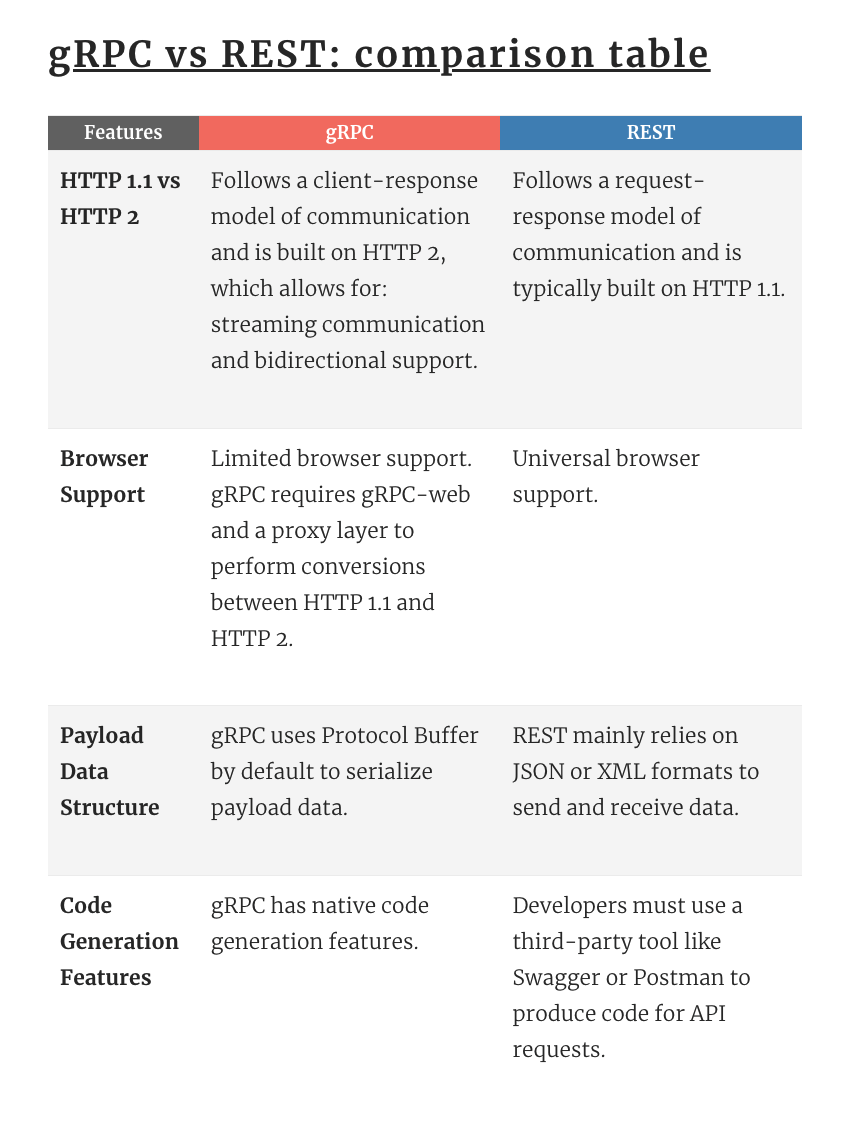
\includegraphics[height=0.3\textheight]{./part/Proyecto_ejecutivo/memoria_constructiva/rpc/img/rpcComparison}
    \caption{gRPC vs REST.\cite{berga_santos_2023}}\label{fig:gRPC vs REST}
\end{figure}
\subsubsection{Infraestructura}\label{subsubsec:infraestructura}
\paragraph{Docker}\label{par:Docker}
    El fichero de definición de una imagen Docker se nombra por defecto como \textit{Dockerfile}.
Expresa la imagen base desde la que se parte, el fichero diseñado usa un sistema operativo debian, y se procede a ejecutar los distintos pasos de instalación de dependencias que se requieren para construir el contenedor.
En un mismo fichero Dockerfile existen distintos stages.
Un stage es cada conjunto de pasos diferenciados por un nombre.
A la hora de levantar el contenedor se puede seleccionar el requerido.
Esto es útil para, en un mismo fichero, especificar si queremos instalar las dependencias para desarrollo o producción.
Así se especifican y ahorran los elementos comunes, que de otro modo habrían de duplicarse y mantener en ficheros separados.
Los stages diseñados son: base, dev, compile y prod.

En la base se instalan los elementos comunes.
Si se especifica dev entonces se instala Golang, el debugger Delve, un usuario para evitar el uso de sudo dentro dicho container y distintas utilidades generales como git, vim como editor de textos y fish como terminal.
Si se construye mediante la etiqueta \textit{compile} se evita la instalación de los elementos de desarrollo y sólo instalamos golang para poder compilar el código.
En prod se usa esa fase primero para compilar.
Luego se parte de la base en limpio y se crea un contenedor con el ejecutable en su interior.
Ahorrando espacio en el contenedor.
Estos pasos pueden apreciarse en la~\cref{lst:dockerfile}.

La infraestructura consta además de una red para hacer visible los contenedores entre si: Manager, clients, base de datos y el proxy para el RPC\@.
La estructura se especifica en un archivo docker-compose.yml .~\cref{lst:dockercompose}.
Habrá un docker-compose.yml aparte para el proxy y la base de datos~\cref{lst:dockercomposegen}.

\phantom{blank}
\vspace{10mm}

\hrule

\begin{lstlisting}[language=docker-compose-2,caption={Docker-compose.yml para cada proyecto golang: Manager, client y control},breaklines=true,label={lst:dockercompose}]
version: "3.9"
services:
    web:
        container_name: go-manager
        build:
            context: .
            dockerfile: docker/Dockerfile
            target: $target
            args:
                GO_VERSION: 19.2
        image: go-manager:19.2-${target}
        ports:
            - "8081:8081"
            - "40000:40000"
        security_opt:
            - "seccomp:unconfined"
        cap_add:
            - SYS_PTRACE
        volumes:
            - .:/app
        tty: true

networks:
    default:
        name: pfm-network
        external: true
\end{lstlisting}


\hrule

\begin{lstlisting}[language=docker-compose-2,caption={Docker-compose.yml de sistemas compartidos y network},breaklines=true,label={lst:dockercomposegen}]
version: "3.9"

services:
  envoy:
    build:
      context: .
      dockerfile: ./envoy/Dockerfile
    image: grpcweb/envoy
    ports:
      - "8080:8080"
      - "9901:9901"
  mysql:
    image: mysql:8.0
    ports:
      - "127.0.0.1:3306:3306"
    container_name: mysql
    command: --default-authentication-plugin=mysql_native_password --general-log=1 --general-log-file=/tmp/mysql.log
    user: "1000:1000"
    environment:
      - MYSQL_ROOT_PASSWORD=$MYSQL_ROOT_PASSWORD
      - MYSQL_DATABASE=$MYSQL_DATABASE
    volumes:
      - pfm-db-data:/var/lib/mysql
volumes:
  pfm-db-data:
networks:
  default:
    name: pfm-network
    external: true
\end{lstlisting}


\hrule

\begin{lstlisting}[language=docker,caption={Dockerfile.yml},breaklines=true,label={lst:dockerfile}]
FROM debian:buster AS base

ARG GO_VERSION
RUN apt update && apt install -y curl

FROM base AS dev

WORKDIR /tmp

RUN apt update && apt install -y build-essential curl vim fish git sudo \
    && groupadd -g 1000 docker-user \
    && useradd -d /home/docker-user -s /bin/bash -u 1000 -g 1000 docker-user \
    && usermod -aG sudo docker-user && echo "docker-user:1234" | sudo chpasswd \
    && mkdir /home/docker-user \
    && chown -R docker-user:docker-user /home/docker-user

USER docker-user
WORKDIR /home/docker-user

RUN URL=https://storage.googleapis.com/golang/go1.${GO_VERSION}.linux-amd64.tar.gz \
        && curl ${URL} -o go.tar.gz  \
        && tar -zxf go.tar.gz  \
        && rm -rf go.tar.gz

ENV GOPATH /home/docker-user/go
ENV PATH $PATH:/home/docker-user/go/bin
ENV CGO_ENABLED 0

RUN go install github.com/go-delve/delve/cmd/dlv@latest
RUN ls -s /home/docker-user/go/bin/dlv /usr/local/bin

WORKDIR /app

FROM base AS compile

WORKDIR /tmp
RUN URL=https://storage.googleapis.com/golang/go1.${GO_VERSION}.linux-amd64.tar.gz \
        && curl ${URL} -o go.tar.gz  \
        && tar -zxf go.tar.gz  \
        && rm -rf go.tar.gz  \
        && mv go /usr/local/go

ENV GOPATH /usr/local/go
ENV PATH $PATH:/usr/local/go/bin
# If you enable this, then gcc is needed to debug your app
ENV CGO_ENABLED 0

WORKDIR /app
COPY ./app .
RUN go build -ldflags "-s -w" -o final.sh

FROM debian:buster AS prod

WORKDIR /
COPY --from=compile /app/final.sh /
CMD ["./final.sh"]
\end{lstlisting}

\hrule
\paragraph{Raspberry}
    Necesitaremos una plataforma donde desplegar el programa de control que disponga de las características necesarias para interactuar con el hardware del  motor de corriente continua y la electrónica de potencia: el puente H. Las soluciones más comerciales son arduino y raspberry. Vamos a poner a prueba además la versatilidad de Golang para compilar el programa para distintas arquitecturas de forma trasparente para el programador. Facilitando su uso con distintas arquitectuas de chip.

Nos decantamos por raspberry por ser una interfaz más amigable de cara al desarrollo y las pruebas del programa. Se entiende que el ámbito del proyecto ya es lo suficientemente complejo y arduino pudiera requerir mayor de esfuerzo debído a no disponer de sistema operativo a la hora de trabajar.

\begin{figure}[H]
    \centering
    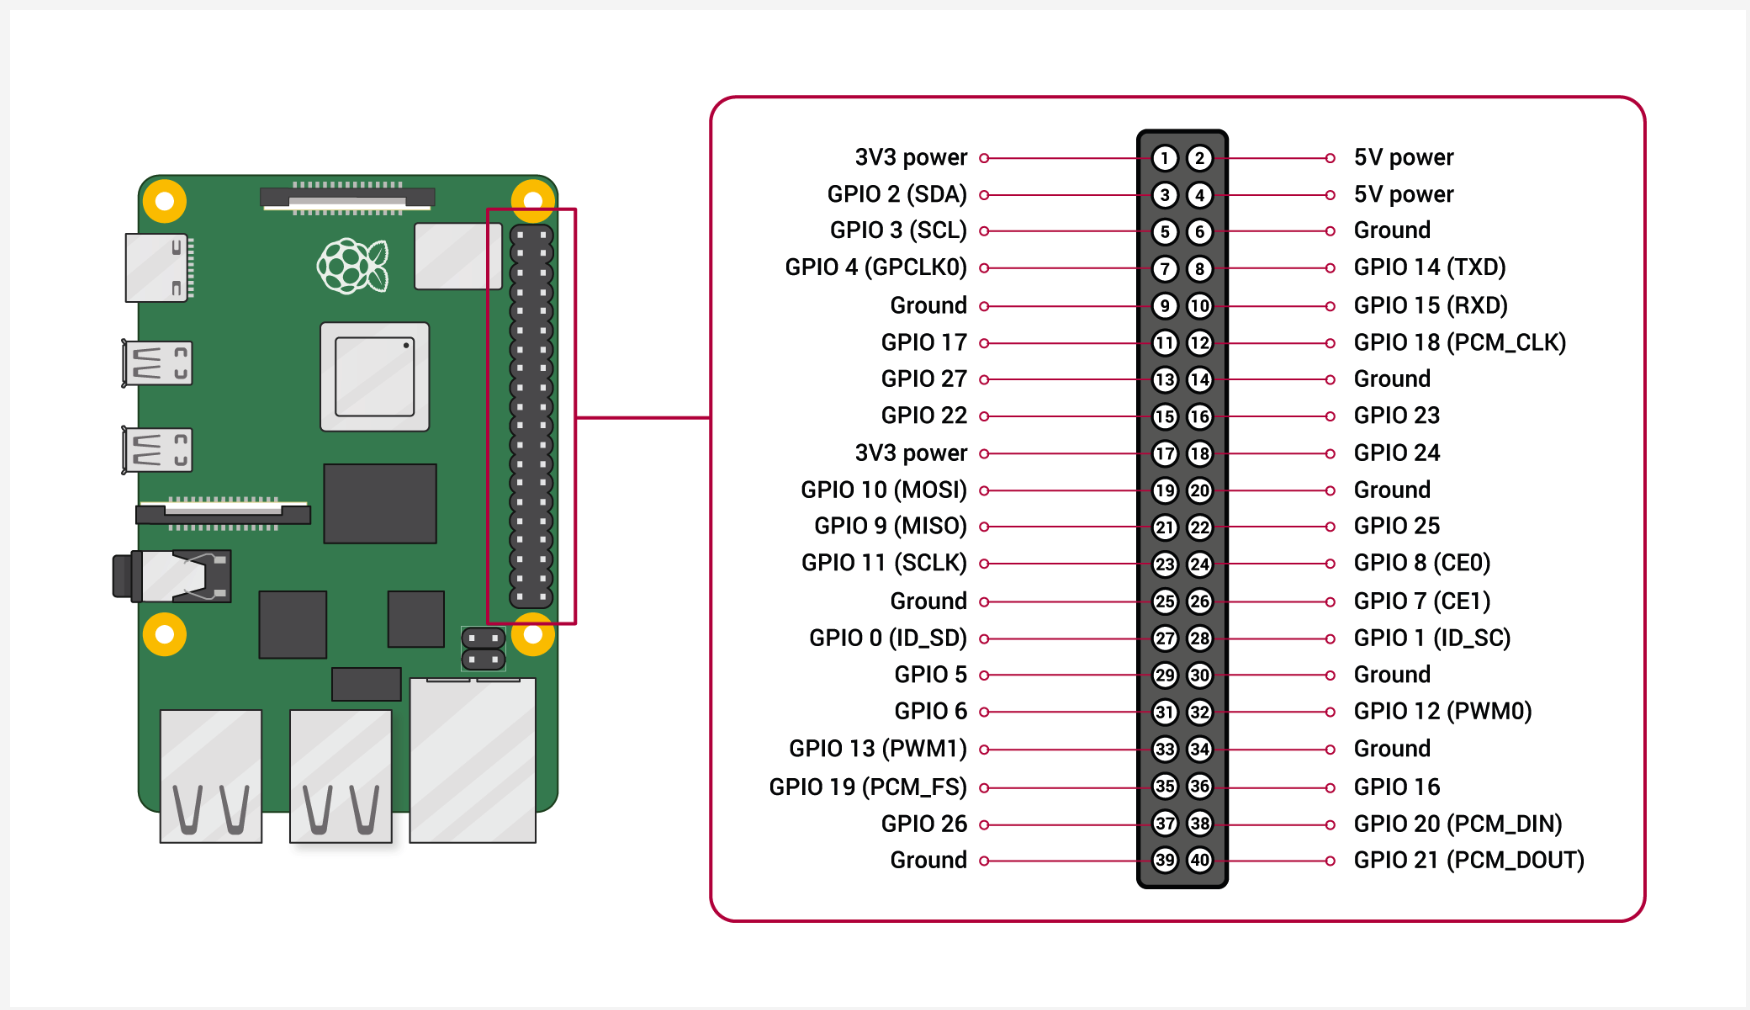
\includegraphics[scale = 0.4]{part/Proyecto_ejecutivo/memoria_constructiva/raspb/img/raspberry}
    \caption[Rasberry schema]{Raspberry schema \\Fuente: }\label{fig:raspberry pins}
\end{figure}

\begin{figure}[H]
    \centering
    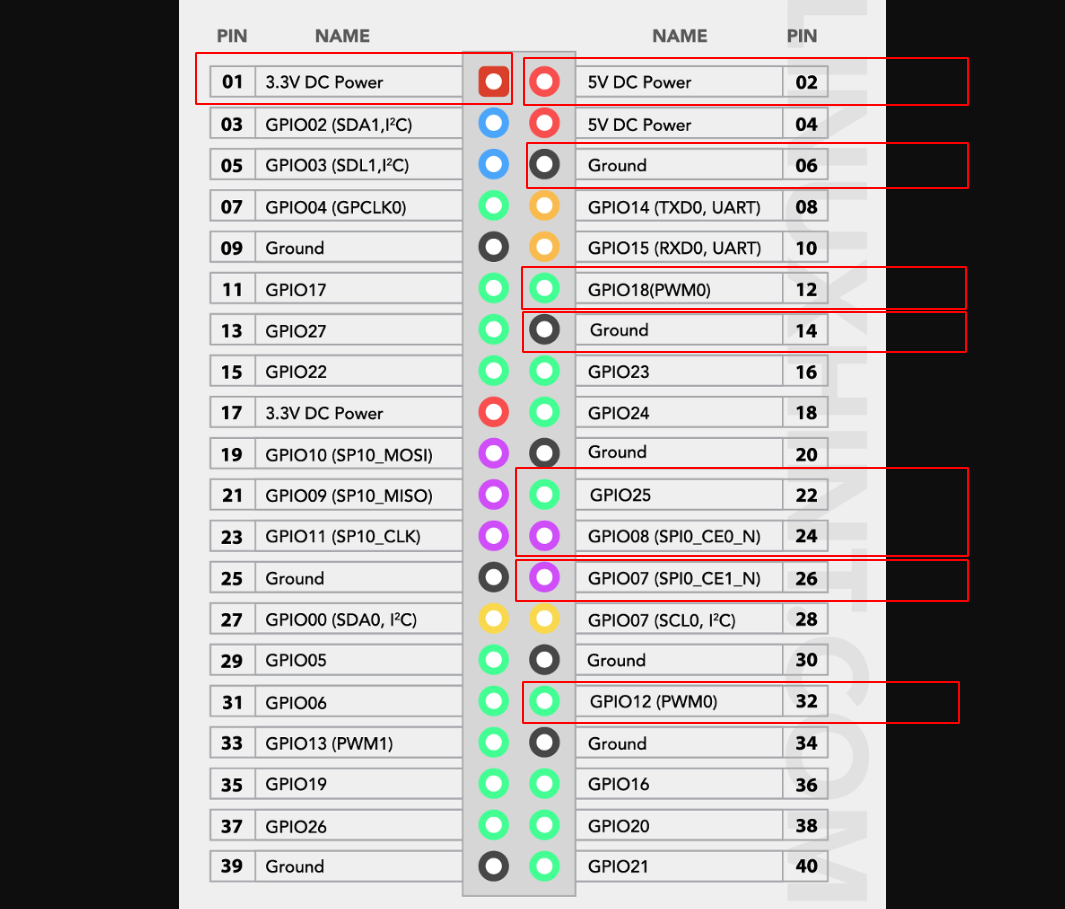
\includegraphics[scale = 0.4]{part/Proyecto_ejecutivo/memoria_constructiva/raspb/img/gpio-pinout-raspberry-pi-01-used}
    \caption[Motor EMG30]{Motor EMG30 \\Fuente: Documento de especificaciones técnicas.}\label{fig:Used Pins}
\end{figure}
\paragraph{Motor CC y puente H}\label{par:docker}
    
El motor seleccionado será el~\cite{EMG30datasheet} Por el conocimiento que se dispone de su uso. En la figura~\cref{fig:EMG Motor} podemos apreciar su aspecto. Para el objeto que nos ocupa cumple con los requerimientos de ser sencillo, barato y disponer de una calidad suficiente.

\begin{figure}[H]
    \centering
    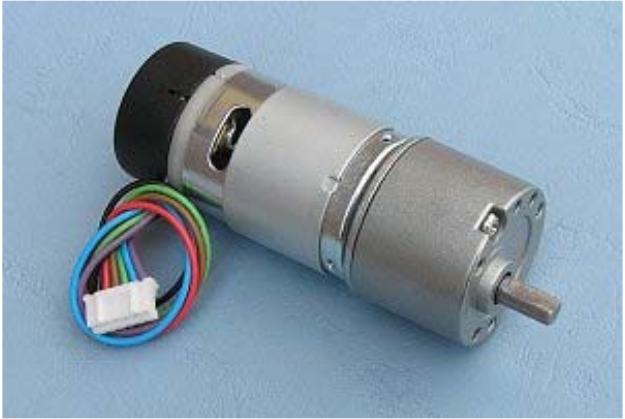
\includegraphics[scale = 0.4]{part/Proyecto_ejecutivo/memoria_constructiva/motor/img/MotorEMG30}
    \caption{Motor EMG30\cite{EMG30datasheet}}\label{fig:EMG Motor}
\end{figure}

Los parámetros que definen sus características más relevantes pueden apreciarse en la Tabla~\ref{tab:EMG30specifications}. El código de colores de las conexiones de las que dispone el motor podemos encontralo en las especificaciones ténicas del mismo. Se extraen en la~\cref{fig:motor connection}


\begin{table}[H]
    \centering
    \begin{tabular}{|l|l|}
        \hline
        Característica & Valor\\
        \hline
        Voltaje nominal & 12 V\\
        \hline
        Torque nominal & 1.5 kg/cm\\
        \hline
        Velocidad nominal & 170 rpm\\
        \hline
        Intensidad nominal & 530 mA\\
        \hline
        Velocidad sin carga& 216 rpm\\
        \hline
        Intensidad sin carga& 150mA\\
        \hline
        Intensidad máxima& 2.5 A\\
        \hline
        Salidad nominal & 4.22 W\\
        \hline
        Pasos por vuelta del codificador& 360 \\
        \hline
        Razón de la reductora & 30:1\\
        \hline
    \end{tabular}
    \caption{Características EMG30 \\ Fuente:\cite{EMG30datasheet}}\label{tab:EMG30specifications}
\end{table}


\begin{figure}[H]
    \centering
    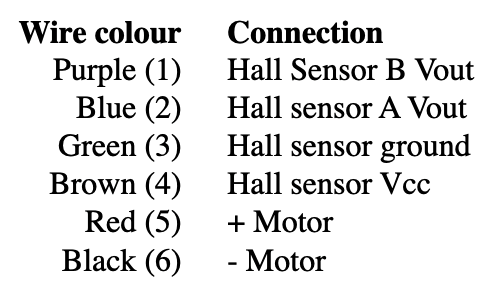
\includegraphics[scale = 0.6]{part/Proyecto_ejecutivo/memoria_constructiva/motor/img/motorConnection}
    \caption{Motor EMG30 \\Fuente: Documento de especificaciones técnicas.\cite{EMG30datasheet}}\label{fig:motor connection}
\end{figure}


    El componente utilizado para ampliar la señal enviada por el Arduino al motor, sirviendo de intermediario entre éste y los motores es el módulo específico para el control mediante PWM de motores con un circuito integrado LMD18200T que soporta hasta tres Amperios. En definitiva es un puente H controlado por PWM.\\

Ha sido elegido por satisfacer todas los requisitos necesarios en nuestra tarea: Precio, voltaje, amperaje y de implementación sencilla. Este módulo podría fabricarse, dado su sencillez, a mano comprando los componentes por separado, sin demasiado esfuerzo.\\
\begin{figure}[H]
		\centering
		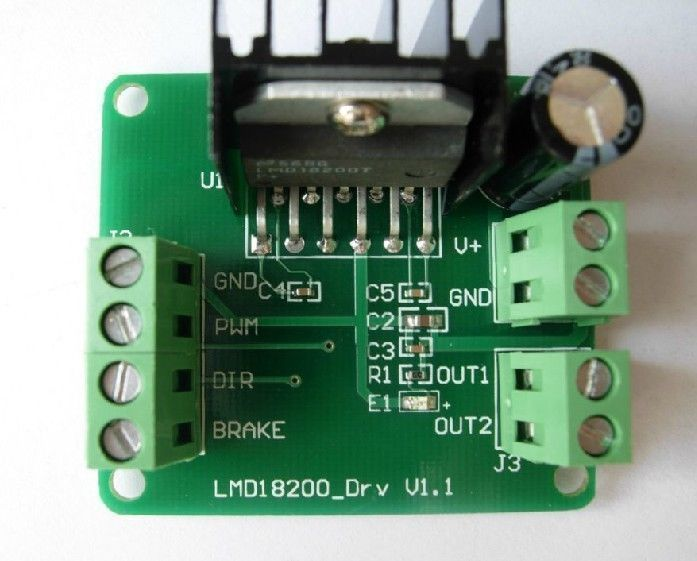
\includegraphics[scale = 0.3]{part/Proyecto_ejecutivo/memoria_constructiva/motor/img/modulopot}
		\caption[Módulo de potencia.]{Módulo de potencia.\\Fuente: \url{http://i.ebayimg.com/}(2014)}\label{fig:figure}
\end{figure}
	
Se aprecian en la figura 6 las entradas y las salidas de las que dispone. De arriba abajo la primera columna es de entradas:

\begin{itemize}
	\item \textbf{GND:} La tierra de la placa de control, en nuestro caso el Arduino.
	\item \textbf{PWM(Pulse width modulation):} la señal del control por ancho de pulsos.
	\item \textbf{Dir:} Señal con el sentido de giro que se desea.
	\item \textbf{Brake:} Freno del motor
\end{itemize}

Y la segunda columna de alimentación y salidas:

\begin{itemize}
	\item \textbf{V+:} Alimentación de 12 voltios.
	\item \textbf{GND:} tierra.
	\item \textbf{OUT1:} Salida de una mitad del puente H.
	\item \textbf{OUT2:} Salida de la otra mitad del puente H
\end{itemize}

La composición del circuito conocido como puente H y su implementación en este módulo viene detallada en el ANEXO donde se referencia al manual del circuito integrado.

		\textbf{Conexión}
El esquema de conexión hacia los elementos con los que interactúa es el siguiente:
\begin{figure}[H]
		\centering
		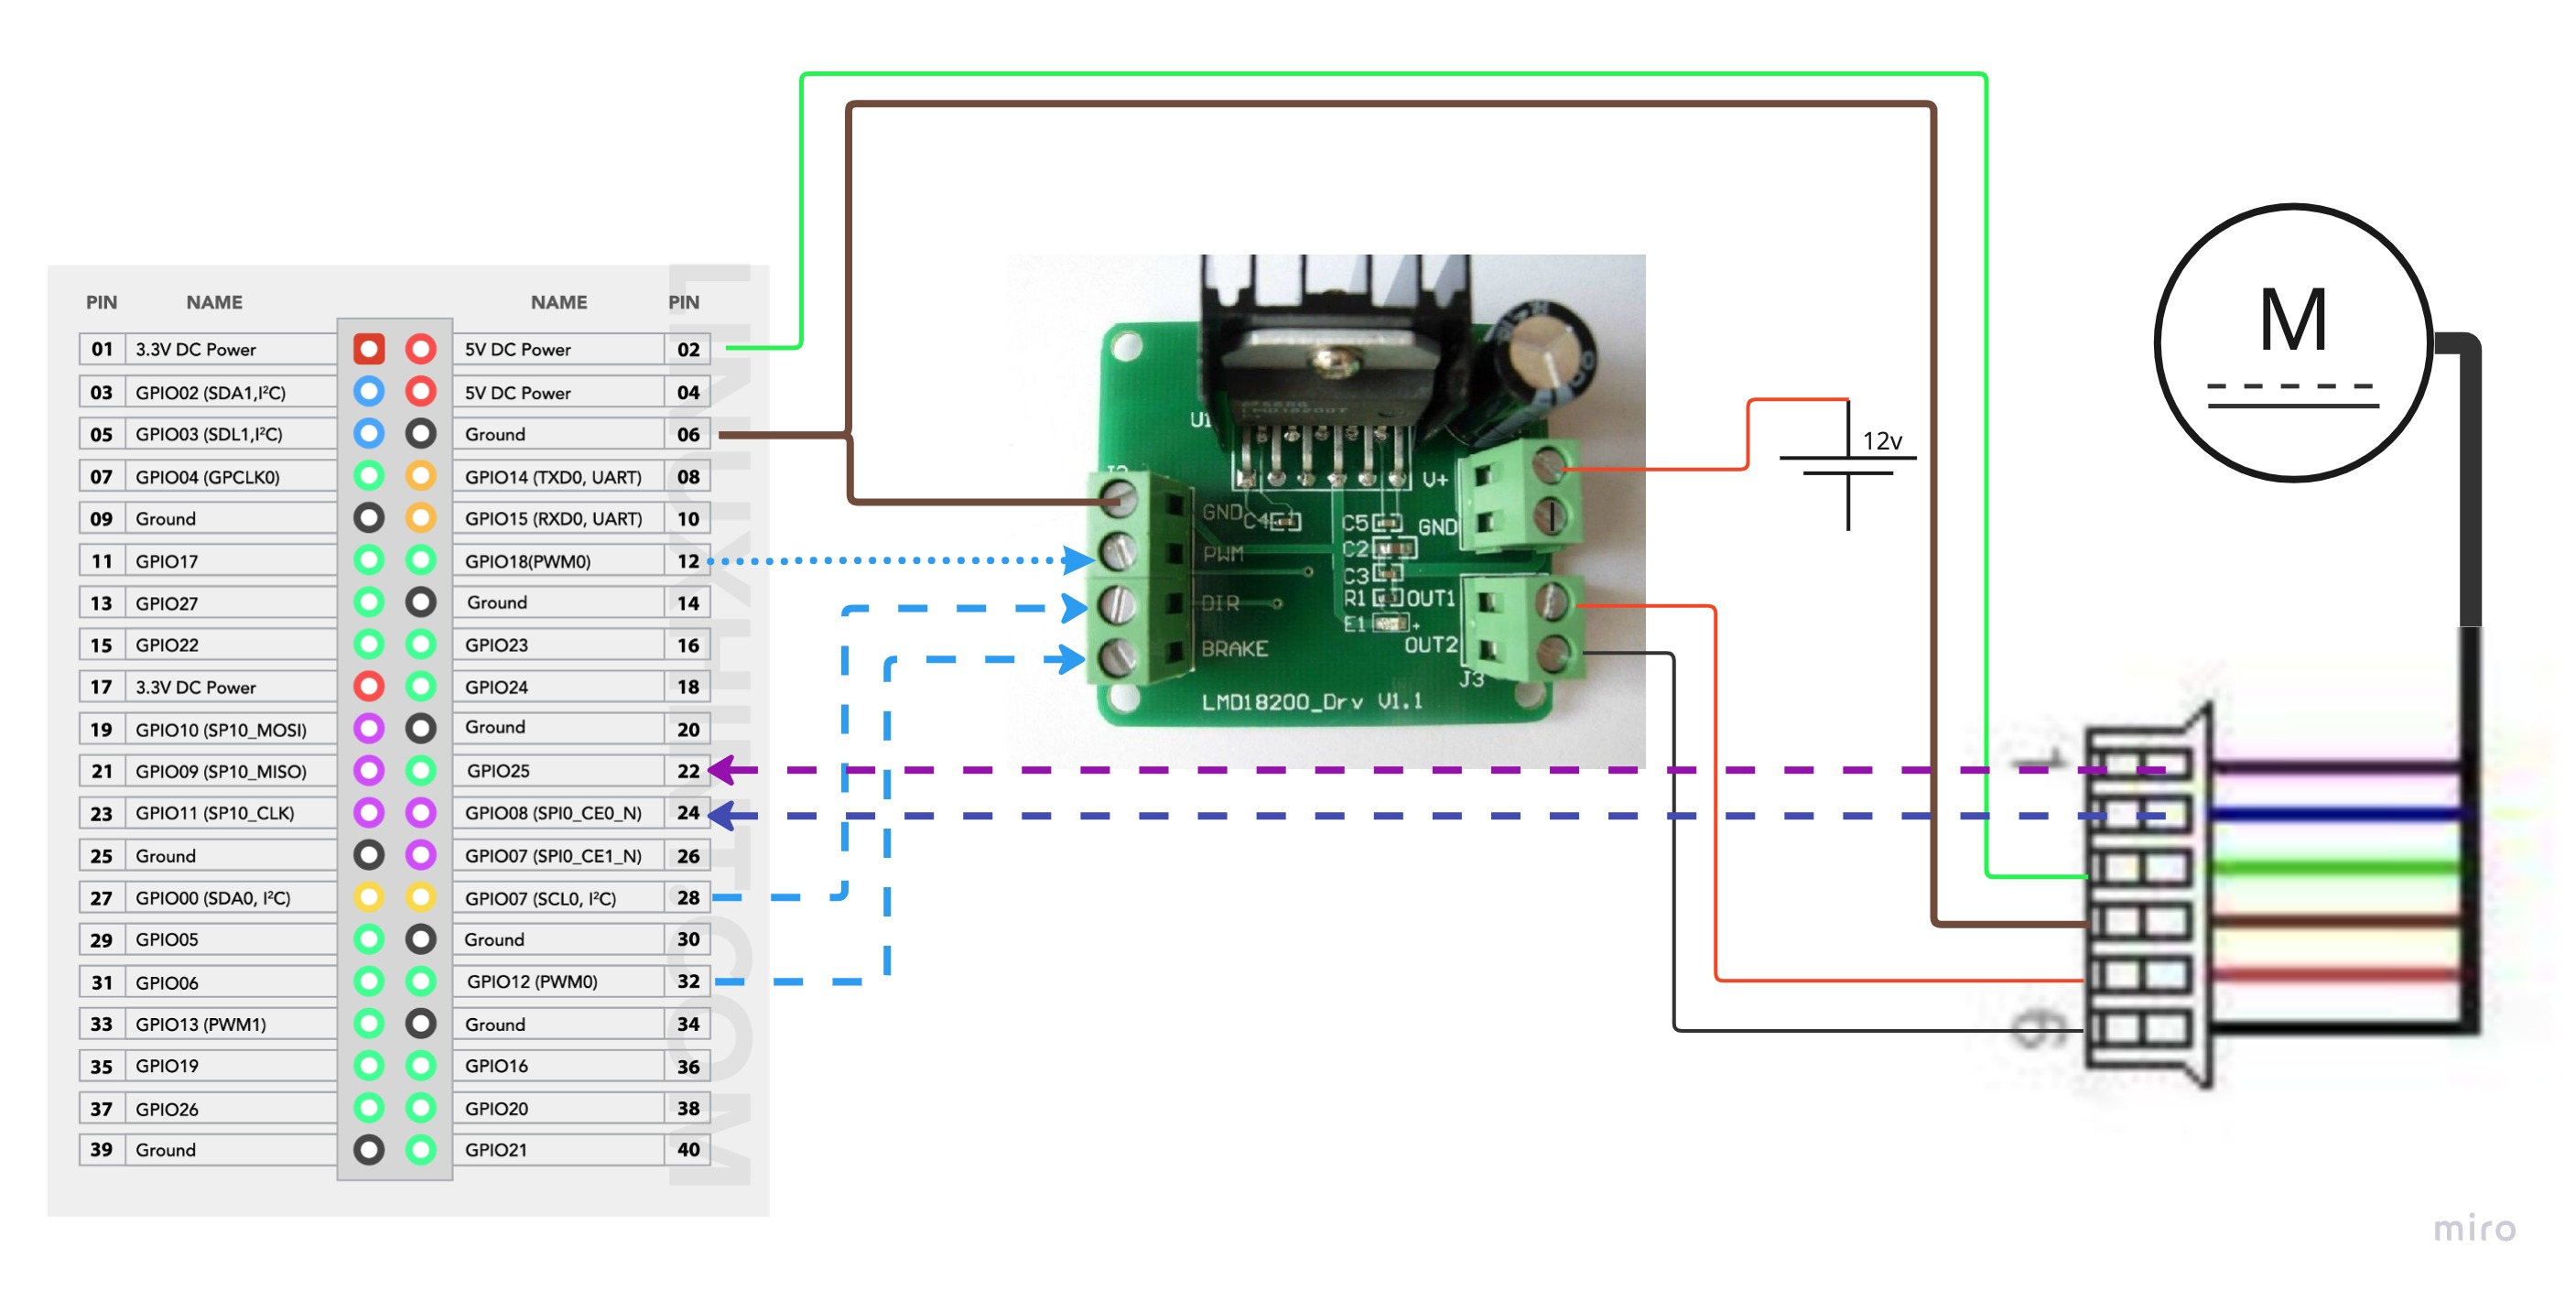
\includegraphics[scale = 0.15]{part/Proyecto_ejecutivo/memoria_constructiva/motor/img/connection diagram}
		\caption[Esquema de conexión del módulo de potencia.]{Esquema de conexión del módulo de potencia.\\Fuente: elaboración propia.}\label{fig:figure2}
\end{figure}
\paragraph{Mysql}\label{par:mysql}
    Para la base de datos escogeremos Mysql por ser también la solución más estandar y que más domino, para no tener que añadir mayor esfuerzo de investigación.
    \begin{figure}[H]
        \centering
        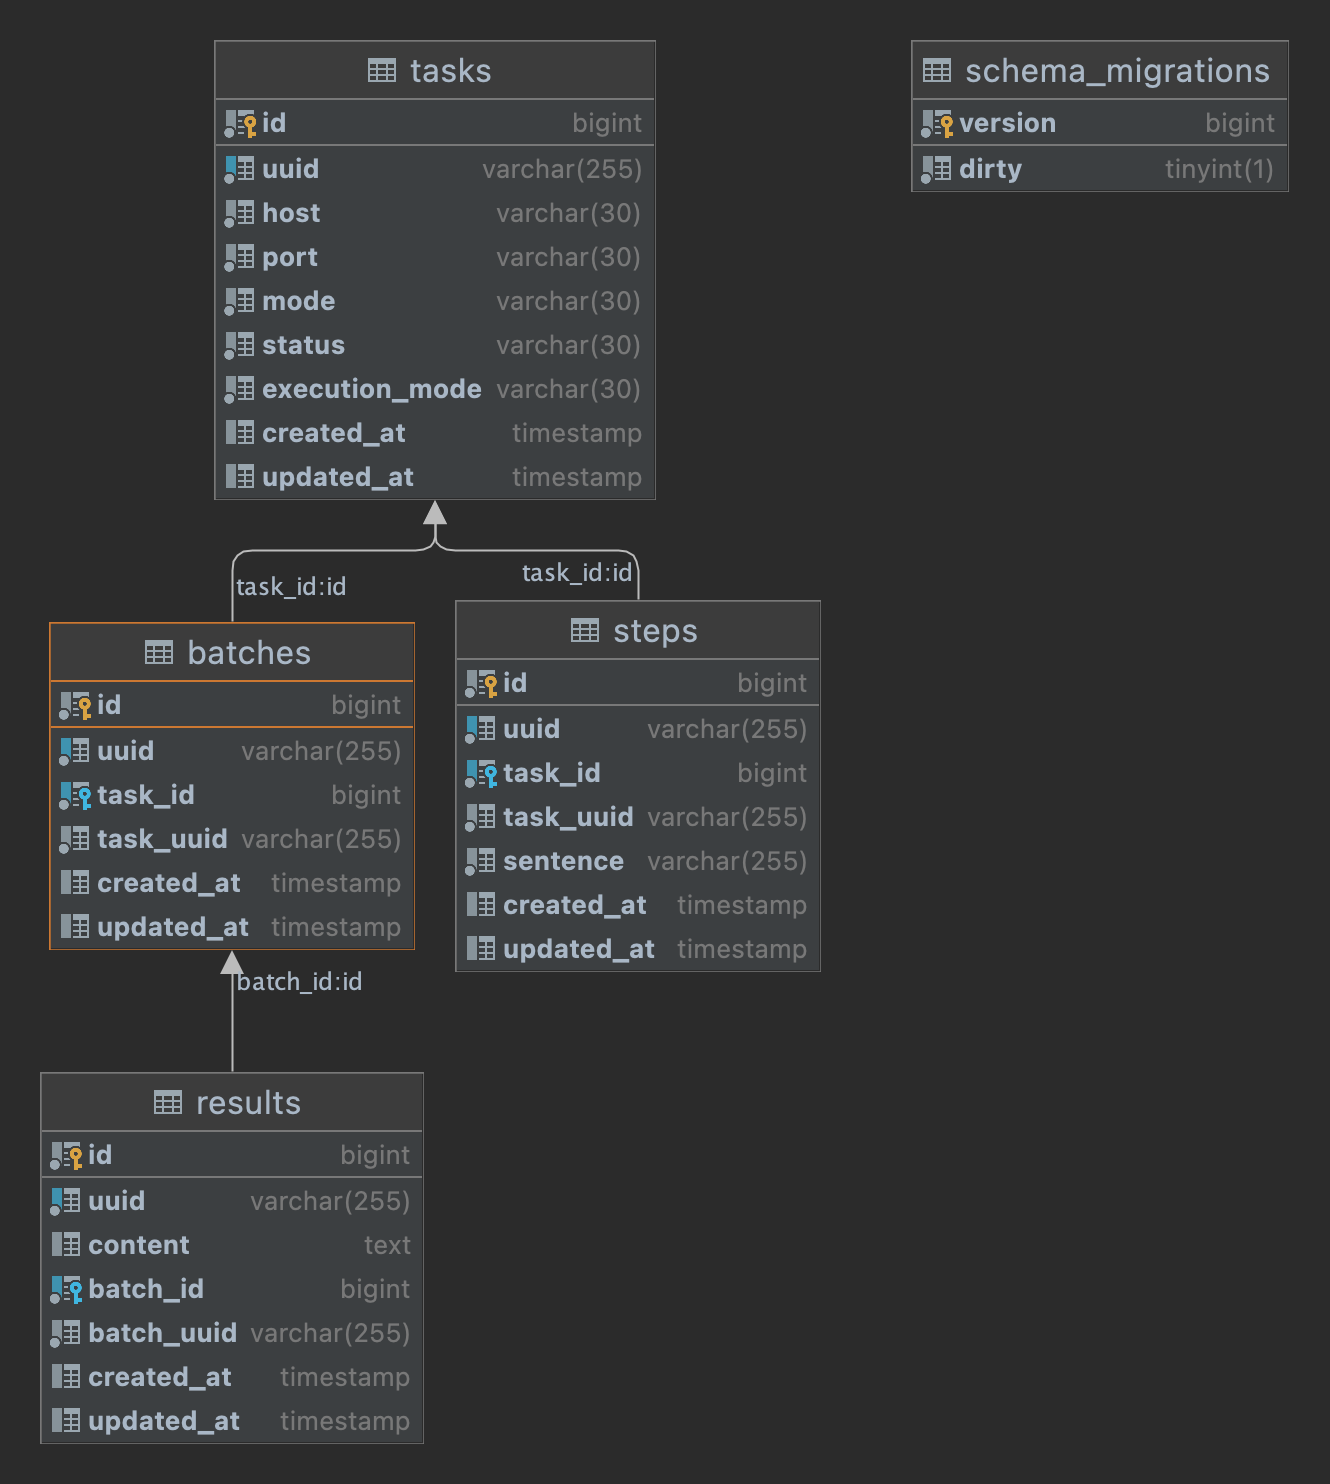
\includegraphics[scale = 0.15]{part/Proyecto_ejecutivo/memoria_constructiva/dbSchema}
        \caption{Esquema de la base de datos}\label{fig:Esquema de la base de datos}
    \end{figure}
\paragraph{CI/CD}\label{par:cicd}
    Archivo githubActions
\subsection{Memoria económica}\label{subsec:memoria-economica}
Uno de los puntos más complicados en el mundo del software es la estimación de costes, tanto de implementación como de mantenimiento. Descuadre entre espectativas-capital disponible-necesidad real. hay problemas por parte del cliente al tener presente el coste real de sus espectativas. hay costes ocultos de mantenimiento, de implementación rápida vs calidad, de malas decisiones por presion en los deadlines. Se quiere plantear esta sección como una estimación del orden de magnitud que puede adquirir el desarrollo de software

    \newpage
    \section{Ejecución}\label{sec:ejecucion}
    \subsubsection{Seguimiento}\label{subsec:seguimiento}

\subsubsection{Memoria explicativa de cambios}\label{subsec:memoria explicativa de cambios}

\subsubsection{Asincronía}\label{subsec:asincronia}

\subsubsection{Planos definitivos}\label{subsec:planos definitivos}

\subsubsection{Encoder}
    \subsubsection{RPC Server streaming}
    \subsubsection{RPC Bidirectional}
\subsection{Problemas RPC en golang}\label{subsec:problemas-rpc-en-golang}

\subsubsection{estado del arte en RPC}
    \subsubsection{decisión: cambio a javascript para fronted}
\subsection{Caso práctico de las ventajas del DDD y arquitectura de capas}
    \subsubsection{análisis del diseño original y propuesta de modificación}
    \subsubsection{modificación ejecutada}
\subsection{Testing}
\subsection{Puesta a punto y resultados}

    \newpage
    \section{Conclusiones}\label{sec:conclusiones}
    El primer punto es que Golang me parece un lenguaje pensado en primer lugar para programas pequeños o scripting. Ahí es donde se puede lucir. Es sencillo y fácil de aprender lo básico necesario para sacarle todo el partido a la asincronía, la limpieza y la sencillez. Tiene paquetes base directamente disponibles sin necesidad de añadir dependencias de tercieros muy potentes que permiten abordar pequeñas tareas con muchas garantías y de forma sencilla. Pequeños endpoints, scripts de procesamiento, algoritmia, paralelismo. Lo cual lo vuelve un candidato muy viable para lo que se suele utilizar python que es el scripting.

Sin embargo, casi todos los proyectos medianos y de grandes dimensiones empiezan siendo pequeños. Los programas que son utilizados y evolucionan, normalmente acaban añadiendo funcionalidades y termina necesitando estructura y diseño para soportar dicho crecimiento, que es lo que ha puesto a prueba principalmente este proyecto. Ahí si que puede sentir el desarrollador que venga de otros lenguaje más maduros que tiene sintaxis un poco enrevesada o que tiende a necesitarse sobreingeniería para montar una estructura lo suficientemente granulada. Una vez se acepta la idiosincrásia del entorno las estructuras que se necesitan para ello, el equivalente a la clase, las interfaces, es cierto que brillan por su sencillez y no dejan espacio para que tienda a enrevesarse.

\textbf{Nomenclatura}

Si bien es cierto que la guia de estílo tiene una filosofía muy bien enfocada y lo suficientemente amplia como para dar libertad, lo que se aprecia en la comunidad es que, precisamente por ese enfoque a scripting, se tiende a elegir variables muy cortas, poco explicativas. Tiene su argumentos para justificarlo siendo el enfoque a realizar diseños pequeños muy modulares

Sin embargo, esto choca de lleno, en mi opinión con la tendencia de abusar a poner mucho código en un mismo fichero y evitar la división en diversos ficheros, lo cual obviamente, como todo tiene sus argumentos a favor juntado con el nombrado de variables que abusan de acrónimos, palabras incompletas y caracteres sueltos abren la puerta a un código dificil de leer, a perder de vista la cohesión, principios y el principio de abertura a funcionalidades y cerrados a cambios.

Mi opinión es que puede tener unos argumentos favorables muy pareceidos a los comienzos de php, javascript o demás lenguajes de scripting. Es ampliamente conocido cómo acaban estas tendencias: ficheros de muchas lineas, variables imcomprensibles, código difícil de leer. Refactorizar un nombre largo y explicativo a uno corto siempre será mucho más sencillo que extraer el significado de una variable nombrada con una letra e intentar darle un nombre mejor. Siempre será más fácil juntar código en un mismo fichero que separarlo. Lo segundo nos obliga a pensar en su cohesión y sus dependencias.

Por lo tanto en este proyecto, que además pretendía ser didáctico, ha abusado de nombres altamente explicativos, sin miedo a caer en la redundancia o el abuso y a dividir cada componente en su propio archivo, algo nada normativo en este lenguaje.

\textbf{Interfaces}

Si bien la teoría apoya la decisión de eliminar la palabra reservada implement para indicar al compilador que una estructura va a implementar una interfaz, de cara al desarrollo lo veo una optimización innecesaria que provoca más problemas de los que puede solucionar. Es cierto que si la signatura de una función se repite debiera ser la misma interfaz y no escribir dos veces la misma interfaz, pero en una arquitectura de capas esto ocurre, ya sea por mal diseño o por que es inevitable en algunos casos, no poder elegir en la implementación de la interfaz con qué paquete está dicho acoplamiento provoca que pueda ser confuso. Además de que al escribir la palabra implement ya avisas a la IDE y al compilador de que quieres que contenga esas funciones y te advierte si no es así.

El argumento a favor más potente que tiene golang es que evitas la necesidad de implementar wrappers de librerias de terceros a las que no quieres acoplarte. Diseñar una interfaz que cumpla esa librería que quieres utilizar ya te aisla de ella. Como es de terceros, si tuvieras que implementarla sólo podrías tocar la librería y poner explicitamente que la implementa, lo cual es absurdo, o tienes que crear una clase que implmentente tu interfaz y hacer una implementación de cada función de la interfaz donde simplemente haces uso de la funcion de la librería, lo cual añade verbosity y complicación.

Mi opinión personal es que no le temo tanto al exceso de código burocrático como los wrappers como a la dificultad de lectura o falta de orden. no tener explicitamente declarada la interfaz creo que favorece dicho desorden.

\textbf{Equivalente de clases vs standard de golang}

Es un punto que al principio me empezó molestando y desconcertando y al que al final más aprecio le he cogido.

Un poco verbose y según el standard de golang un poco antiparttern. Pero al final mi conclusión es que no utilizaría structs sueltos en casi ningún punto. A lo mejor muy encapsulados en una función que enfrente una algoritmia complicada y requiera estructurar datos de una forma rápida inline

\textbf{Paquetes y división del código en golang}

Comentar que no hay manera de ocultar ciertas cosas al exterior. El objeto de los Aggregate es ocultar al exterior los VO y las Entity que contienen.

\textbf{Testing}

Estandar del test unitario al lado de la clase hace que tengas imports raros en el dominio ademas de todo el codigo para mockear en medio de tu codigo de producción

Puede venir bien para gestión de equipos que vengan de scripting porque sentirán mayor orden y estructura
puede ser complicado para gente que venga de lenguajes con un orden más estándar como js,php puede costar adaptarse a la idiosincraisa del lenguaje y pasar por el aro

\textbf{Gestión del proyecto}

La arquitectura y el diseño que se han empleado busca que el propio código sea la documentación, ya que, si bien un entregable es requisito imprecintible para un tfm en la vida real el mantenimiento de esta documentación se vuelve inviable. Si bien es interesante un minimo de documentación que requiere la gente no técnica para entrar en el conocimiento del dominio y el mantenimiento de la documentación de la interfaz de los casos de uso.

Hay mucha teoría al respecto de la gestión de proyectos de software, pero muchas veces partir de un estandar ya definido y bien depurado como es la presentacion de proyectos puede ser un paso, la cantidad de veces que me han agradecido presetnar un documento inicial que ponga en contexto, aclare, de materia firme a la que acogerse para ir definiendo el proyecto no es muy tipica en el mundillo


    \newpage
    \section{References}\label{sec:references}
    \bibliographystyle{plain}
    \bibliography{/Users/enrikerf/workspace/thesis/out/refs}
\end{document}